\newchapstyle
\chapter{Experimental methods}
\label{chap:experiment}

\epigraph[0pt]{
	Remember, kids, the only difference between screwing around and science is writing it down.
}{Adam Savage, quoting ballistics expert Alex Jason, in the 2012 MythBusters episode \textit{Titanic Survival}~\cite{savageOriginOnlyDifference2015}}

\blfootnote{
	\color{title}
	The recipes and procedures regarding graphene heterostructures are based on extensive prior work of the group of Dr.~Srijit Goswami at QuTech, TU Delft, and were further developed in close collaboration with Dr.~Nikos Papadopoulos.
	%
	Recipes on DC bias cavities were developed together with Dr.~Mark Jenkins.
	%
	Fabrication was carried out in the Kavli Nanolab cleanroom of TU Delft.
}


\begin{abstract}
A significant, if not the major portion of an experimental physics thesis consists of the countless hours being spent on the (sometimes seemingless never ending) loop of device fabrication and device measurement.
% 
This chapter serves to give an insight into the methods and techniques being used to assemble functioning devices, together with a few tips and tricks that might be of use to other experimenters.
% 
While the backbone of this thesis was the use of the Kavli Nanolab Delft cleanroom, one of the biggest academic cleanrooms on the European continent, and all measurement presented in this thesis were performed in state-of-the-art dry dilution refridgerators, the methods are nonetheless extendable to smaller-scale laboratories.
\end{abstract}

%% Start the actual chapter on a new page.
\newpage

\section{Device fabrication}
\label{sec:fabrication}



\subsection{The art of making encapsulated graphene devices}

Fabrication of graphene Josephson junctions is a tedious process:
% 
in contrast to integrated circuits, where the active materials are homogeneously deposited over an entire substrate, which enables massive parallel processing, the best graphene devices to date are not fabricated using scalable techniques, but rather each device is manually assembled and crafted.
%
This requires significant efforts, since no two devices have the same exact shape, which often results in slightly different properties between devices.


The most promising wafer-scale graphene fabrication is achieved by chemical vapor deposition of single layer graphene on copper foils~\cite{zhangReviewChemicalVapor2013,linBridgingGapReality2018}.
% 
However, only recently have such deposited films exhibited sufficiently low defect densities for high quality transport, which would otherwise result in inferior device quality~\cite{banszerusBallisticTransportExceeding2016a,neumaierIntegratingGrapheneSemiconductor2019}.
% 
Additionally, device quality can be reduced by contaminations that are often encountered when transferring the graphene layer from its growth to the final substrate.
% 
Finally, even in the cases where transferred graphene itself only exhibits low defect and residue densities, patterning it into the final device shape almost exclusively contaminates it, most often via organic resist residues.

Since single layer graphene (SLG) is really only a single atom thick and thus all electronic transport takes place at its surface, contaminations on either side will result in charge carrier scattering and degrade the device performance.
% 
Till this day, the vast majority of devices with highest electronic quality, exhibiting phenomena such as ballistic transport, hydrodynamics, or superconductivity, rely on single layer graphene manually exfoliated from bulk graphite crystals~\cite{mayorovMicrometerScaleBallisticTransport2011b,bandurinNegativeLocalResistance2016a,caoCorrelatedInsulatorBehaviour2018,caoUnconventionalSuperconductivityMagicangle2018a}.


Additionally, it is often required to tune the carrier density in the graphene layer, for which a gate electrode separated by a dielectric is needed.
% 
Because of the single-layer nature of graphene, it conforms very well to any surface roughness and is very sensitive to trapped charges in the dielectric layers.
%
Significant efforts were put into removing the substrate entirely, thus freely suspending graphene.
%
This, in conjunction with device annealing to burn off fabrication residues, can result in remarkably high-quality samples~\cite{duApproachingBallisticTransport2008a,rickhausBallisticInterferencesSuspended2013,mizunoBallisticlikeSupercurrentSuspended2013a,kiHighQualityMultiterminalSuspended2013,maurandFabricationBallisticSuspended2014,rickhausGateTuneableBeamsplitter2015,rickhausGuidingElectronsFewMode2015}.
% 
However, such devices are highly fragile and fabrication can be tedious~\cite{rickhausElectronOpticsBallistic2015}.
%
On the other hand, finding an inert dielectric would ease fabrication needs.
%
To this end, Dean \textit{et al.}~\cite{deanBoronNitrideSubstrates2010} realized the use of hexagonal Boron Nitride (BN) as the (until now) best dielectric and capping layer for graphene devices, showing vast improvements with respect to device mobility.


Like graphene, BN has a hexagonal lattice, albeit consisting of two sub-lattices of boron and nitride atoms with a lattice mismatch of \SI{1}{\percent} to graphene.
% 
BN can be exfoliated from bulk crystals to thin insulating films of arbitrary layer number and signifcantly lower surface roughness than any other dielectric, making it a perfect match for graphene encapsulation.
% 
The highest quality BN crystals, i.e. the ones exhibiting the lowest charge defect density, are made by high pressure synthesis by Kenji Watanabe and Takashi Taniguchi at the \textit{National Institute for Material Sciences} (NIMS), Japan~\cite{taniguchiSynthesisHighpurityBoron2007,zastrowMeetCrystalGrowers2019}.

As confirmed by atomic force and scanning tunneling microscopy, SLG on BN exhibits significantly lower roughness compared to samples on \ce{SiO2}, until then the standard dielectric for graphene devices.
% 
In addition, variations in the local density of states of SLG on BN is reduced by a factor ten, while charge fluctuations are suppressed by a factor 100, as compared to SLG directly on \ce{SiO2}~\cite{xueScanningTunnellingMicroscopy2011,deckerLocalElectronicProperties2011}.
% 
Complete screening of any trapped charges in the dielectric layer is possible with gate electrodes made of graphite instead of conventional metals~\cite{ponomarenkoTunableMetalInsulator2011,ametNovelPhenomenaDriven2014}.
%
BN encapsulation even enables ballistic transport in very high quality CVD graphene devices~\cite{banszerusBallisticTransportExceeding2016a}.


Flake transfer procedures have since paved the way for the assembly of so-called van der Waals heterostructures, named so due to the van der Waals forces holding the flakes together.
%
This has allowed for all kinds of exfoliatable crystals to be stacked, which enabled a new method of studying emergent phenomena such as induced spin orbit coupling, ferromagnetism or superconductivity~\cite{geimVanWaalsHeterostructures2013a,novoselov2DMaterialsVan2016}.
%
In this PhD thesis, however, we limit ourselves to the use of only SLG and BN to study induced superconductivity in the SLG.
%
Even so, assembling a heterostructure of BN-G-BN, with subsequent patterning, and deposition of gate metals and dielectrics results in an extensive and long process, with processes varying between most research groups.
% 
In the following, we will detail the fabrication procedure used in the course of this thesis that resulted in the best measured devices.

\subsubsection{Substrate cleaning and flake exfoliation}

All BN-G-BN heterostructures are based on SLG and few-layer BN exfoliated from bulk highly oriented pyrolithic graphite (HOPG) and \textit{NIMS} BN, respectively.
% 
Identifying flakes of suitable thickness is done by estimating the layer number and thickness from optical images.
% 
For optimal contrast~\cite{blakeMakingGrapheneVisible2007b}, we used silicon substrates with \SI{285}{\nano\meter} of dry chlorinated thermal \ce{SiO2}, diced into \SI{6x6}{\milli\meter} pieces from \SI{4}{inch} wafers from \textit{NOVA Electronic Materials}.
% 
Details on dicing parameters are given in Sec.~\ref{sec:fab-packaging}.


As mentioned earlier, any organic residues that come in contact with graphene will very likely lead to inferior device performance.
% 
Specifically, after dicing the chips, they need to be cleaned extensively in order to remove any leftovers from the dicing resist.
% 
To this end, diced chips are placed in a teflon holder and transferred through four \SI{50}{\milli\liter} glass beakers filled with acetone, acetone, isopropyl alcohol (isopropanol, IPA) and IPA, each time ultrasonicated for \SI{5}{\minute}.
% 
The chips can either be blow-dried one by one using high-pressure nitrogen gas, or by rinsing the teflon holder with the chips still on it in three water baths and placing it on a petri dish in an oven.
% 
To remove acetone and IPA residues, the chips are ultrasonicated for \SI{5}{\minute} in nitric acid and blow-dried after rinsing in water.
% 
We found that an additional soft oxygen plasma to functionalize the \ce{SiO2} surface (\SI{200}{sccm} of \ce{O2}, \SI{600}{\watt}, \SI{2}{\minute}, no cage in a \textit{PVA Tepla 300}) just before, i.e. not more than \SI{15}{\minute} prior to, flake exfoliation increased flake exfoliation yield, regardless of graphene or BN.

While there already exist fully automized exfoliation-to-heterostructure stations~\cite{masubuchiAutonomousRoboticSearching2018a}, we performed all of the following steps manually.
%
Flake exfoliation is achieved by manually thinning down bulk crystals until micron-sized flakes of only one or two (SLG, BLG) or a few tens of layers (BN) thickness are left on a chip.
% 
We estimate that there are as many different ways of flake exfoliation as there are researchers working on this procedure.
% 
The procedure that worked best for us concerning BN exfoliation consists of placing individual BN crystallites (approximately a few \SI{100x100x100}{\micro\meter} in volume) on a piece of \textit{Scotch} tape \textit{"Magic"} or \textit{Nitto} tape\footnote{Nitto Processing Tape SWT20+ REACH R 280X100, bought from TELTEC GmbH}, and subsequently folding over said piece of tape numerous times, such that one acquires a closed layer of thin BN crystallites.
% 
In the case of graphene, we would peel off a preferably closed film of graphite from a single \SI{1x1}{\centi\meter} HOPG crystal with a piece of tape, followed by subsequent folding of the piece of tape until we acquired a homogeneous, yet closed film of thin graphite.


Once satisfied with the tape template, we used pre-cut \SI{8x8}{\milli\meter} pieces of clean tape to peel off crystals from the template and press the side with crystals on the small piece of tape onto a previously cleaned substrate.
%
After having kept pressure applied for approximately \SI{30}{\second}, we transferred the substrate with the tape still on to a hot plate and left the chip sit for \SIrange{2}{5}{\minute}.
% 
We found highest flake densities for temperatures of \SI{50}{\celsius} for \textit{Nitto} and \SI{100}{\celsius} for \textit{Magic} tape.
% 
Finally, the chip was transferred off the hot plate, left to cool for \SI{1}{\minute} and the tape was gently peeled off, while holding the substrate in place with a pair of tweezers.
% 
During this process, no further pressure should be applied to the tape as this usually results in lots of tape residues on the chip.


The process of exfoliation turns out to be a tradeoff between getting as many flakes as possible, and getting the lowest tape residues possibles.
% 
\textit{Magic} tape has a higher adhesive strength, thus resulting in a higher flake density and predominantly large flakes (i.e. larger than \SI{20x20}{\micro\meter}) compared to \textit{Nitto} tape.
% 
On the other hand, this comes at the cost of more tape residues on both substrate and the individual flakes.
% 
Tape residues can lead to enhanced charge carrier scattering of graphene films, thus severely limiting device quality.
% 
Additionally, they increase the chance of bubble formation (see below), thus limiting the available sample space.
% 
Tape residues can be entirely removed by thermal annealing at \SI{400}{\celsius} in  an \ce{Ar + H2} atmosphere.
% 
However, it proved extremely difficult to pick up or transfer flakes treated in this manner for heterostructure assembly.
% 
While we found that annealing at temperatures below \SI{300}{\celsius} was still compatible with flake transfer, significantly less tape residues were removed this way.
% 
It is thus advisable to omit thermal annealing until the first lithography step and instead settle on a slightly lower exfoliation yield.

\subsubsection{Heterostructure assembly}

For assembling our BN-G heterostructures, we used the original transfer setup of Castellanos-Gomez \textit{et al.}~\cite{castellanos-gomezDeterministicTransferTwodimensional2014d}, upgraded with a heater stage capable of fast heating and cooling cycles between room temperature and \SI{200}{\celsius}.
%
The stage was additionally equipped with a small center hole to which a pump was attached via tubing.
%
This allowed us to fix the substrates to or from which flakes were transferred via vacuum, avoiding glue residues from commonly used sticky tape which are notorious to remove after high temperatures.
%
Heterostructures were assembled with a modified version of the procedures developed by Pizzocchero \textit{et al.}~\cite{pizzoccheroHotPickupTechnique2016a} and Zomer \textit{et al.}~\cite{zomerFastPickTechnique2014b}.
% 
BN-G-BN structures are formed by repeated pick-and-place of SLG and few-layer BN (flake thickness between \SIrange{10}{50}{\nano\meter}).
%
The process makes use of the change in viscoelasticity of an adhesive film on top of an elastic cushion of polydimethylsiloxane (PDMS), which is stuck to a microscope glass slide.
%
Heating this transfer template above the glass transition temperature $T_\text{g}$ of the polymer expands the cushion and allows the adhesive film to become viscous, thus conforming and adhering strongly to flakes covered by it.
%
Cooling below $T_\text{g}$ then solidifies the polymer and flakes will be picked up by lifting the transfer template.

We used two different adhesive films, either polypropylene carbonate (PPC) or polybisphenol carbonate (PC).
%
We prepared the PPC solution by dissolving PPC acquired from \textit{SigmaAldrich}\footnote{Poly(propylene carbonate), average $M_\text{n}\sim50,000$ by GPC. SigmaAldrich product no. 389021, CAS 25511-85-7, MDL MFCD00197919} at a \SI{15}{\percent} weight ratio in anisole\footnote{Anisole, ReagentPlus\textsuperscript{\textregistered}, \SI{99}{\percent}. SigmaAldrich product no. 123226, CAS 100-66-3, MDL MFCD00008354} at \SI{50}{\celsius}, while stirring with a fish magnet until everything was properly dissolved.
%
The PC\footnote{Poly(Bisphenol A carbonate), average $m_\text{W}\sim 45,000$ by GPC. SigmaAldrich product no. 181625, CAS 25037-45-0, MDL MFCD00084476} was dissolved in chloroform\footnote{Chloroform, anhydrous, $\geq\SI{99}{\percent}$, contains \SIrange{0.5}{1.0}{\percent} ethanol as stabilizer. SigmaAldrich product no. 288306, CAS 67-66-3, MDL MFCD00000826} at a \SI{6}{\percent} weight ratio.
%
While PPC requires lower working temperatures than PC, thus making it easier to align template and substrate, we have observed that temperatures above \SI{110}{\celsius} resulted in fewer bubbles at the flake interfaces during transfer.
%
The advantage of PC over PPC is that it is a much stronger adhesive, so the intermediate flake delamination (step \ref{flake-delam}) can be skipped.
%
However, it needs to be kept in a fridge in order to not degrade, and cannot be spin-coated on the PDMS layer, whereas PPC can.
%
Instead, a droplet of PC is placed on a \SI{20x20}{\milli\meter} glass coverslip.
%
A second coverslip is dropped on the first one, thus spreading the droplet in between.
%
With care, but in a swift motion, we pull the top glass piece off, thus leaving behind a thin film of PC on the bottom glass slide, which can be peeled off using a piece of tape and placed on the PDMS stamp.

The adhesive film was placed on a droplet of PDMS which was stuck to a glass slide.
%
Both glass slide and chip could be individually moved with micrometer screws.
%
The following steps describe our typical working process for achieving high-quality interfaces using the PPC method:

\begin{enumerate}
	\item Align the top BN flake with the center area of the PDMS/PPC template.
	%
	Lower the glass slide such that the PPC touches the substrate.
	%
	Take care that the PPC does not yet cover the flake, but touches down less than \SI{100}{\micro\meter} away from it.
	%
	\item Increase the stage temperature above \SI{55}{\celsius}.
	%
	The PDMS/PPC will expand and cover the flake, and adhesion between BN and PPC increase significantly.
	%
	\item Turn off the stage heater and wait for the stage to cool below \SI{40}{\celsius} (possibly with the help of a nitrogen gun).
	%
	At this stage, the adhesion between BN and PPC should exceed that of BN and substrate.
	%
	Now lifting the glass slide should rip the flake off the substrate.
	%
	If at this stage the intended flake did not get picked up, repeating the process by heating to \SIrange{80}{90}{\celsius} and then cooling down should result in a much higher yield, at cost of longer waiting times for the stage to cool down.
	%
	\item Place the chip with the graphene flake on the stage and align the flake with the BN on the glass slide below now.
	%
	Slowly lower the glass slide and set the stage temperature to \SI{110}{\celsius}. 
	%
	The hot air and deflected slide will make it difficult to align the two flakes, so extra care has to be taken at this step.
	%
	Once the stage has reached \SI{110}{\celsius}, bring stage and glass slide in contact as slowly as possible until the interface passes the Gr and BN, preferably letting the expanding PDMS do the work.
	%
	\label{assembly-start}
	%
	\item Increase the stage temperature to \SI{120}{\celsius} and then retract the glass slide, thus delaminating the top BN on the graphene flake.
	%
	\label{flake-delam}
	\item Anneal the Gr/hBN stack at \SI{170}{\celsius} for \SI{15}{\minute}.
	%
	\item Place PPC/PDMS glass slide above the chip, turn off the stage heater and bring the polymer in contact once the temperature is below \SIrange{70}{80}{\celsius}.
	% 
	\item Once the temperature drops below \SI{40}{\celsius}, retract the glass slide.
	%
	The Gr/hBn stack should get lifted off the substrate.
	%
	\label{assembly-stop}
	%
	\item For assembling the BN-G-BN sandwich, repeat steps \ref{assembly-start} - \ref{assembly-stop}.
	%
	If needed, transfer the sandwich to another substrate.
\end{enumerate}

For flake transfer using PC, we follow the above steps, except that the transfer takes place at a base temperature of \SI{110}{\celsius} instead of \SI{40}{\celsius}, and to activate the adhesion to PC, heating to \SIrange{130}{140}{\celsius} instead of \SIrange{80}{90}{\celsius} is required.


\begin{figure}
	\centering
	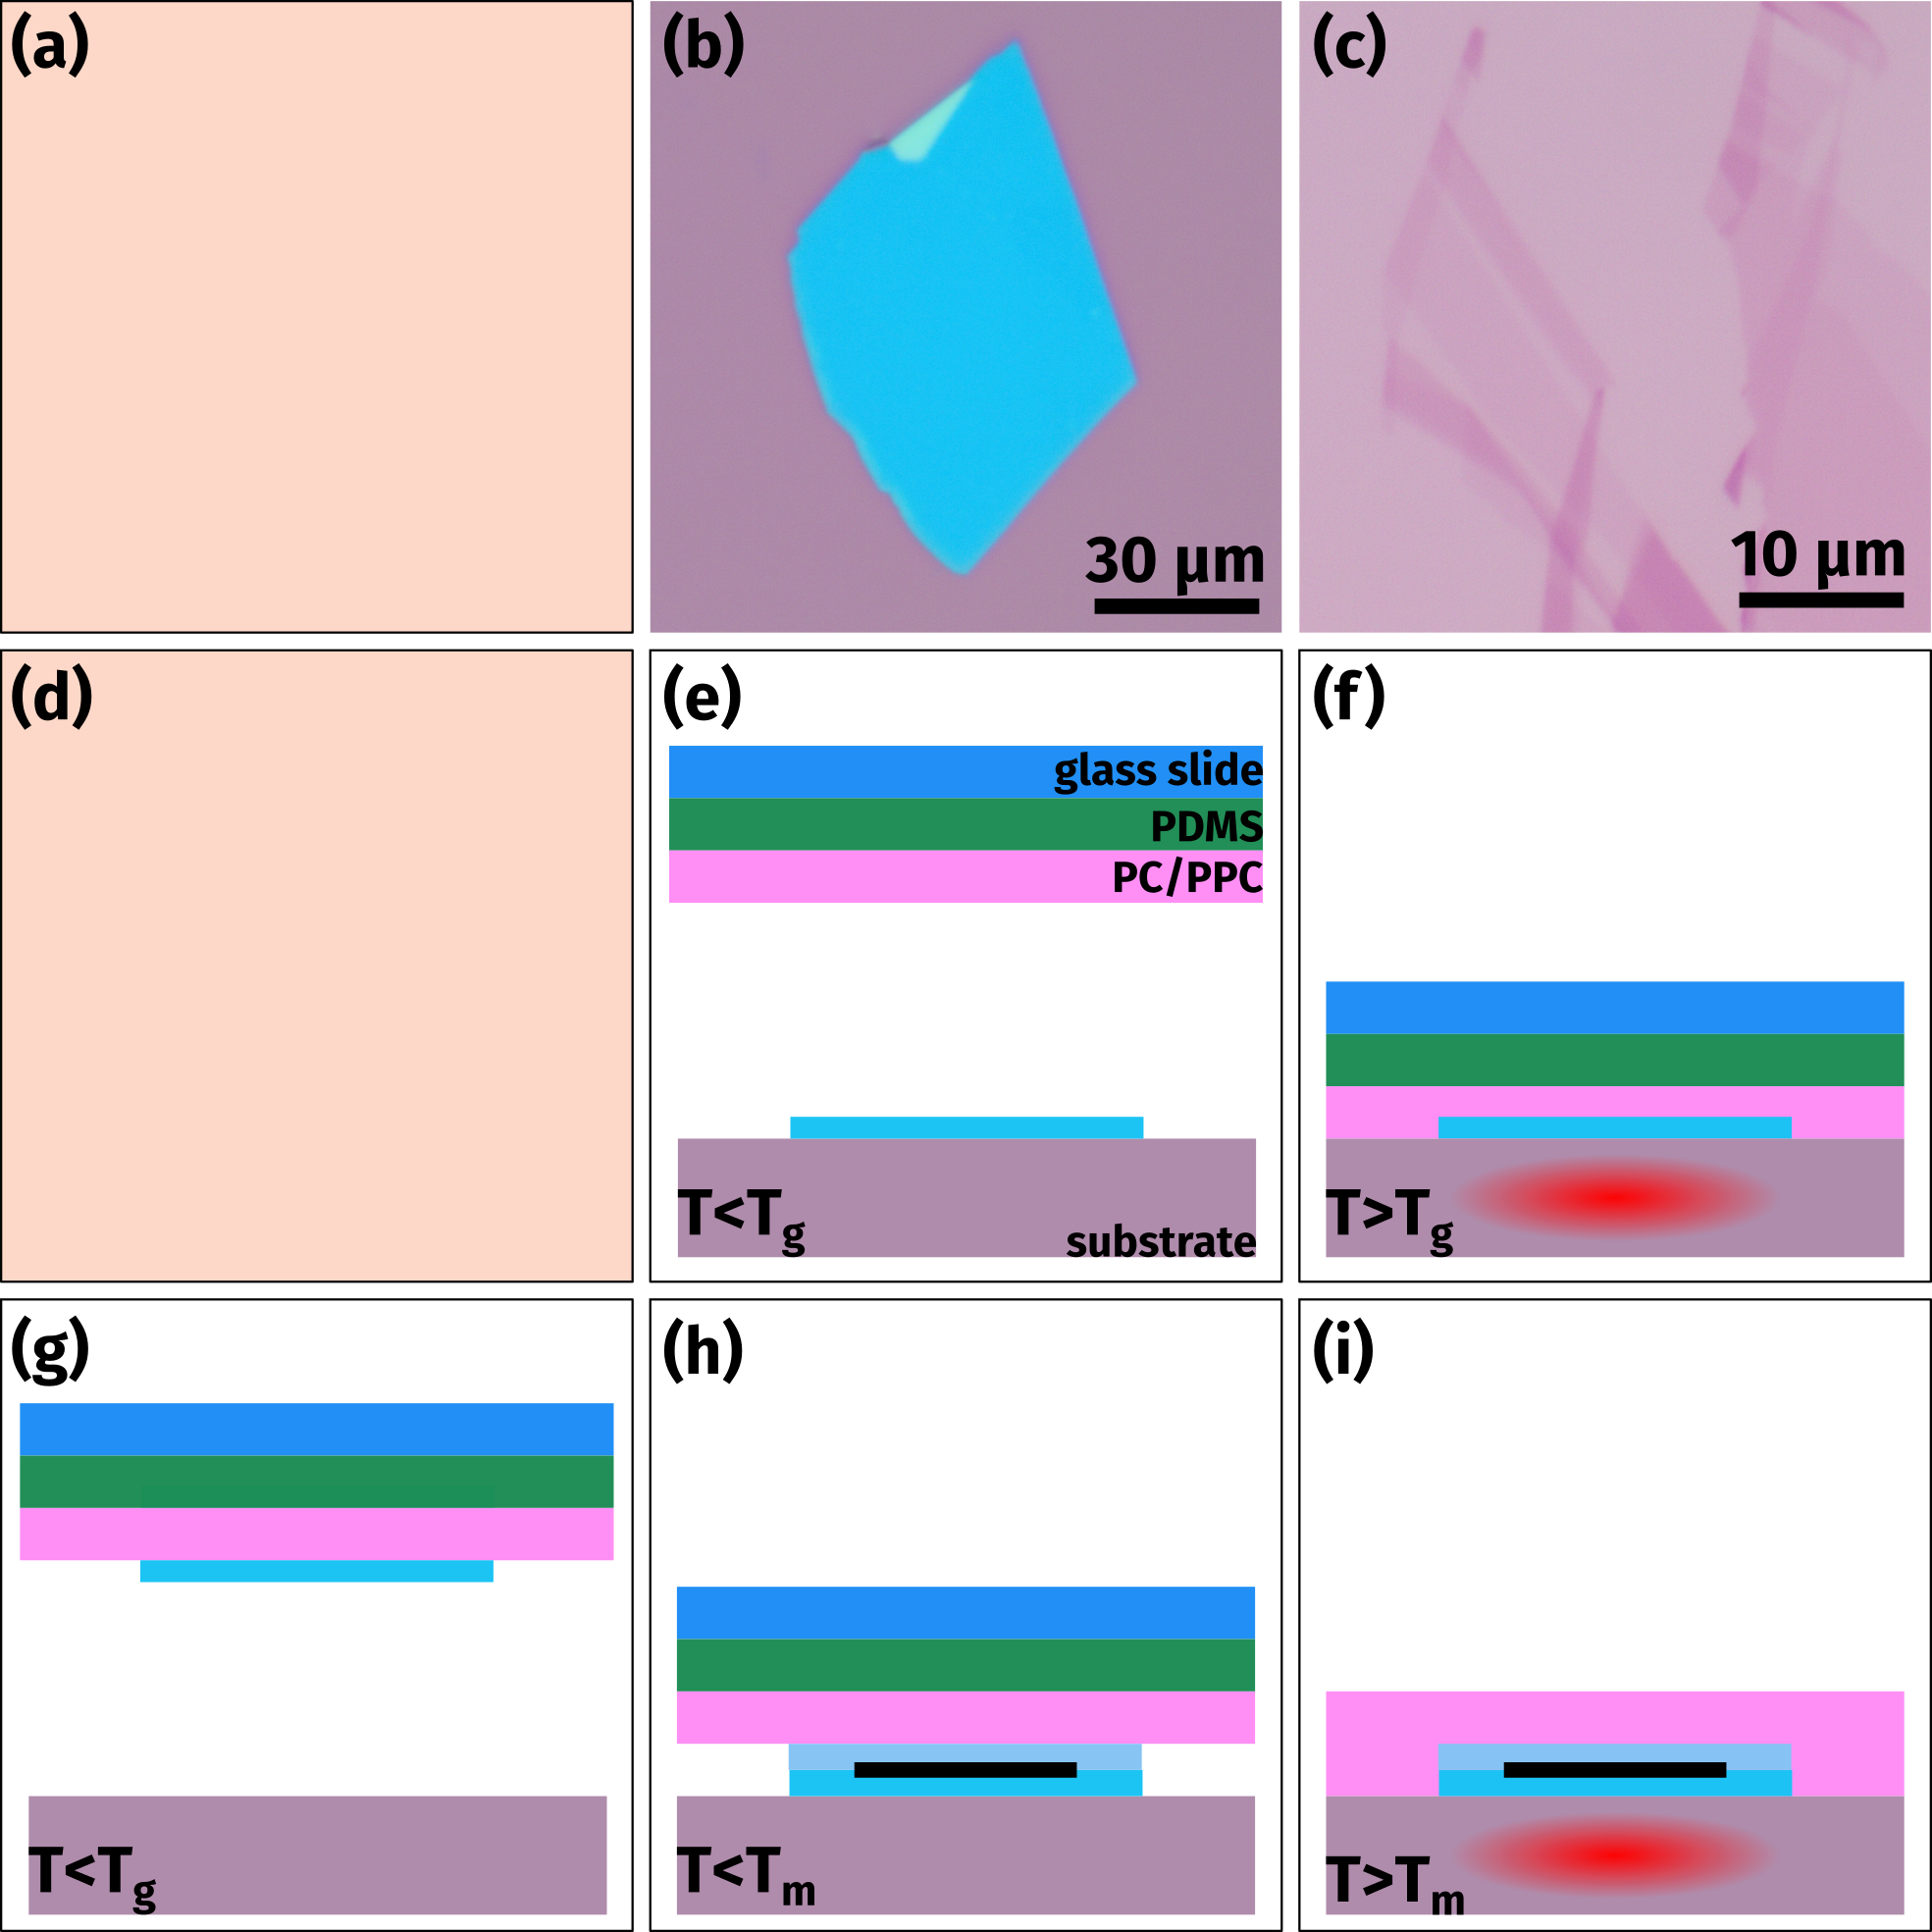
\includegraphics[]{{chapter-experimental-methods/figs-fabrication/fab-heterostructures.svg}.png}
	\caption{
		\textbf{From bulk crystals to van der Waals heterostructures.}
		% 
		\textbf{(a)} Bulk crystals of graphite, together with a piece of wafer adhesive tape used to thin down these crystals by repeated folding and opening of the tape.
		% 
		The tape is pressed on a \SI{6x6}{\milli\meter} piece of silicon with \SI{285}{\nano\meter} \ce{SiO2} to enhance the optical contrast for monolayer graphene.
		%
		Figure adapted from~\cite{papadopoulosMesoscopicTransport2D2019}.
		% 
		\textbf{(b)} Optical microscope image of a BN flake of approximately \SI{30}{\nano\meter} thickness.
		% 
		\textbf{(c)} Optical microscope image of a thin flake of graphite, exhibiting regions of single and multilayer graphene.
		% 
		\textbf{(d)} Photograph of a glass slide with PDMS covered with a spun-on layer of PPC (approximately \SIrange{1}{2}{\micro\meter} thick), aligned to a silicon substrate mounted on the transfer stage.
		% 
		\textbf{(e-i)} Typical sandwich assembly cycle for creating multi-layered van der Waals heterostructures.
		% 
		\textbf{(e)} Polymer brought in contact with exfoliated flake on substrate at room temperature.
		% 
		\textbf{(f)} Heating substrate above glass transition temperature $T_\text{g}$ enhances the adhesion of the flake to the polymer significantly above the adhesion to the substrate.
		% 
		\textbf{(g)} Subsequent cooling of the substrate leads to stiffening of the polymer.
		% 
		Combined with rapid lifting of the glass slide, usually solely induced by the thermally shrinking polymer, lifts the flake off the substrate.
		% 
		By repeating steps \textbf{(e)}-\textbf{(g)}, multiple flakes can be stacked on top of each other.
		% 
		\textbf{(h)} In order to deposit the finished heterostructure on a final substrate, the heterostructure is brought in contact with the substrate at room temperature, and the stage heated above the melting temperature of the polymer.
		% 
		Slow lifting of the glass slide leads to the structure remaining on the substrate, while the polymer can either remain fully stuck to the PDMS, or also remain on the substrate.
		% 
		\textbf{(i)} Polymer residues can be removed in organic solvents such as anisole, NMP, PRS3000 or chloroform.
	}
	\label{fig:fabheterostructures}
\end{figure}

\subsubsection{Challenges of heterostructure assembly}

Compared to interfacing van der Waals heterostructures with DC circuitry, numerous challenges arise for integration with RF devices.
%
RF circuits in coplanar architecture, such as the ones in this thesis, need a metallic ground plane around the conducting lines, separated by micron-sized gaps.
%
Due to the long-range interaction of electromagnetic fields, fabrication residues of any kind (metallic, dielectric, organic) should be avoided as much as possible to ensure reliable circuit operation.


That being said, the nature of flake transfer always introduces contaminations:
%
for one, the polymer used for transfer has very strong adhesion to the metal areas of the shunts, ground planes and center conductors.
%
While during stack assembly on oxidized silicon, the polymer would only touch the substrate at the start, when attempting to delaminate the heterostructure on the pre-patterned substrates, the polymer often ripped off the PDMS carrier and would also get delaminated, cf. Fig.~\ref{fig:fab-hetero-challenge}(a).
%
Additionally, van der Waals crystals have strong adhesion to the metals used in our work, which resulted in a number of residual flakes on the final chip surrounding the intended heterostructure.
%
A long soak in NMP was able to remove the polymer at least visibly, but residual flakes had to be etched away in a separate step.


On the other hand, flake adhesion to the substrate itself was found to vary from good to extremely poor:
%
We found that BN-G-BN stacks would often get washed away due to unsufficient adhesion to sapphire substrates during processing.
%
Due to the low adhesion of BN to sapphire and silicon nitride, many stacks were washed off the final substrates when dissolving the polymer.
%
While the transfer yield of heterostructures on sapphire and silicon nitride was only as low as \SI{50}{\percent} and \SI{0}{\percent}, respectively, we did not observe this behaviour on silicon and silicon oxide surfaces, (cf. Fig.~\ref{fig:fab-hetero-challenge}(b)), where all delaminated flakes would stick.
%
Note that even adhesion promotion using HMDS (hexamethyldisilazane, \ce{[(CH3)3Si]2NH}) did not improve this issue.


When stacking flakes on top of each other, hydrocarbon gases and water, usually covering all surfaces in ambient conditions, can get trapped in between flakes~\cite{haighCrosssectionalImagingIndividual2012}, similar to air pockets encountered when placing protective covers on flat surfaces such as phone screens or windows.
%
These bubbles can cluster together, reaching pressures of up to \SI{1}{\giga\pascal}~\cite{khestanovaUniversalShapePressure2016,ghorbanfekr-kalashamiDependenceShapeGraphene2017} and resulting in local pseudomagnetic fields in excess of \SI{300}{\tesla}~\cite{levyStrainInducedPseudoMagneticFields2010}.
%
Bubbles are hence undesirable since they pose strong charge carrier scattering centers.
%
Nevertheless, high substrate temperatures, both during and after assembly, can mobilize these gasses, allowing them to clear up large sample spaces by accumulating along flake defects.
%
We have occasionally observed bubbles piercing the top BN and escaping from the stack when annealing the heterostructures at temperatures above \SI{300}{\celsius}.

For these reasons, every single gJJ has to be designed by hand, since it is important to place the structure to be fabricated in an area without bubbles present in order to obtain a high-quality device.
%
After stack placement on the final chip, we took several optical and atomic force microscope images to determine the graphene location with respect to alignment marks, and to identify bubble-free areas, cf. Fig~\ref{fig:fab-hetero-challenge}(b).
%
These combined images are loaded into the CAD software (we highly recommend \textit{KLayout}~\cite{KLayoutLayoutViewer}, or alternatively \textit{LibreCAD}~\cite{LibreCADFreeOpen}) to design the electrodes and gates for the gJJ, as shown in Fig~\ref{fig:fab-hetero-challenge}(c).

\begin{figure}
	\centering
	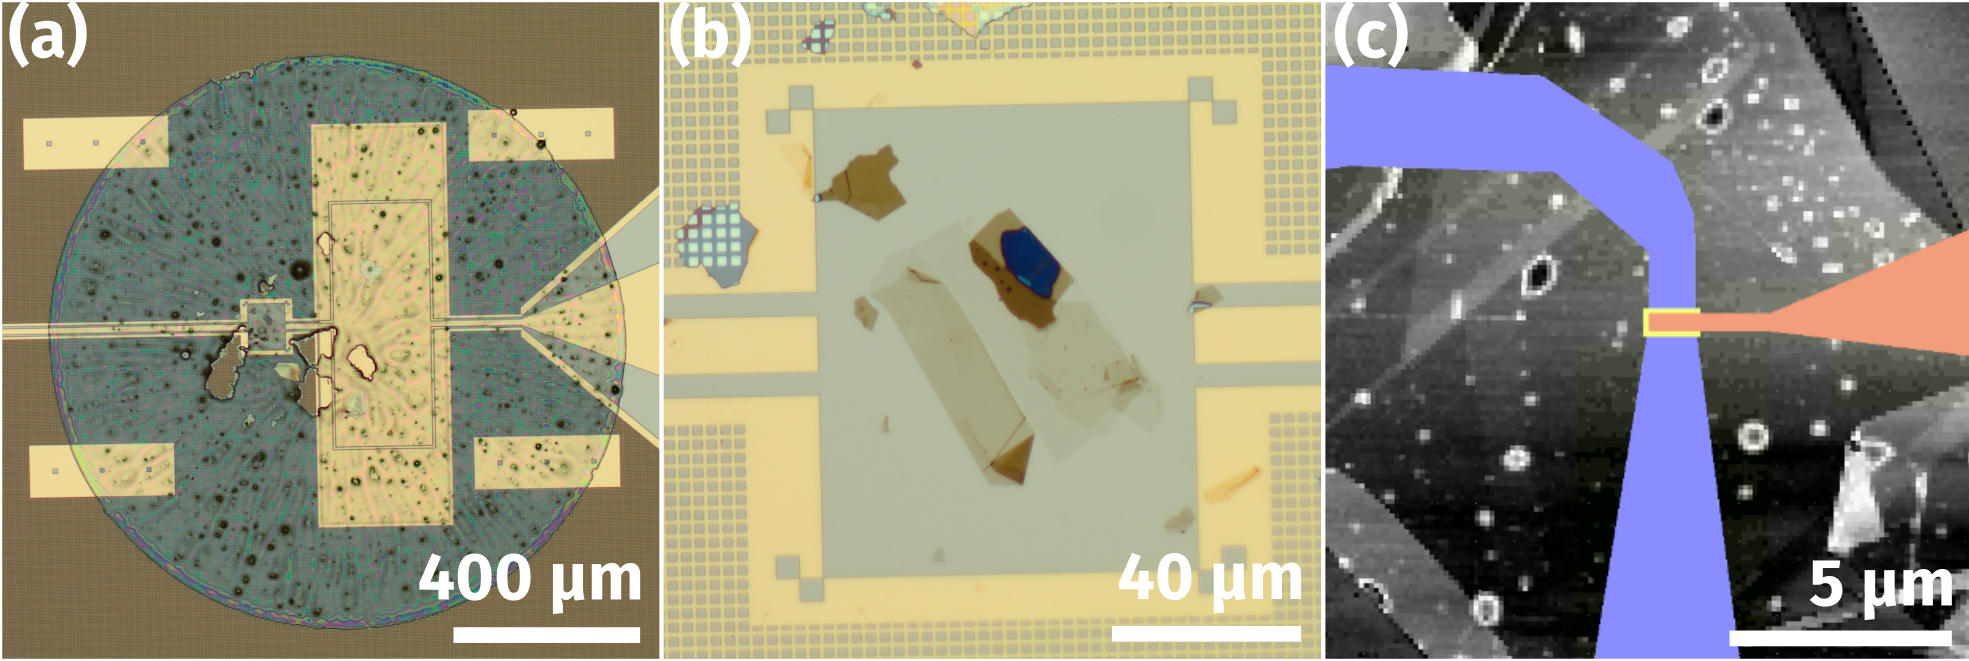
\includegraphics[]{{chapter-experimental-methods/figs-fabrication/fab-hetero-challenge.svg}.png}
	\caption{
		\textbf{Fabrication issues associated with van der Waals assembly.}
		% 
		\textbf{(a)} Due to the good adhesion of the polymer to metal surfaces, after flake deposition the polymer would often get delaminated and the chip needs to be thoroughly cleaned using wet chemistry solvents.
		% 
		\textbf{(b)} Due to the high adhesive strength of the PC and PPC, residual flakes around the assembled heterostructure are delaminated on the chip, requiring additional etching steps to clean the chip of these dielectrics.
		% 
		\textbf{(c)} AFM image (greyscale) of a heterostructure assembled via the PC method.
		% 
		Due to the significantly slower expansion of the polymer, gas and water molecules at the interfaces between the flakes are pushed towards the edges and fewer, but larger pockets are formed.
		% 
		Overlaid with the AFM image is the CAD file with contacts in blue, top-gate in red and gate dielectric in yellow, to design the metal layers with respect to the flake position.
	}
	\label{fig:fab-hetero-challenge}
\end{figure}

\subsubsection{Device patterning and arising challenges}\label{sec:fabgJJ}

Since the gJJ have to be individually designed are not fabricated scalably, we chose to first pattern the RF circuitry on either large silicon chips, or \SI{2}{inch} sapphire wafers, and subsequently transfer the BN-G heterostructures on the final substrate, where they are patterned into the gate-tunable gJJ.
%
Fabrication was carried out in the class 10000 (ISO 7) cleanroom of the \textit{Kavli Nanolab Delft}, which offers class 100 (ISO 5) wet bench areas for sample processing.
%
While the RF circuits could also have been fabricated using photolithography, we patterned all devices using electron beam lithography with either one of the \textit{Raith EBPG 5200} or \textit{5000+}.
%
Dry-etching was done using \textit{Leybold Heraeus Fluor} reactive ion etchers, dielectric deposition with PECVD in an \textit{Oxford Instruments PlasmaPro 80}.
%
Superconductors were deposited in sputtering systems from \textit{AJA International, Inc.} and \textit{Alliance Concept}.

The graphene Josephson junctions were fabricated using the etch-fill technique pioneered by Wang \textit{et al.}~\cite{wangOneDimensionalElectricalContact2013b}, with added top-gates as in Refs.~\cite{nandaCurrentPhaseRelationBallistic2017,schmidtBallisticGrapheneSuperconducting2018}.
%
Compared to fabrication on oxidized silicon, we encountered numerous challenges during fabrication that needed to be addressed before samples could be processed reliably.
%
We chose NbTiN as superconductor for the contacts to graphene after the MoRe target in our lab ran empty, and since the use of NbTiN was well established in the neighboring group of Leo Kouwenhoven~\cite{popinciucZerobiasConductancePeak2012,mourikSignaturesMajoranaFermions2012}.

We found that for ebeam lithography on sapphire substrates, a conductive charging layer on top of the bilayer PMMA in the form of Electra 92 (AllResist AR-PC 5091) was crucial to create high-resolution patterns, such as Josephson junctions with length by width of \SI{0.5x5}{\micro\meter}.
%
Without a conductive layer, the resist would consistently be exposed in the center of the junction, leading to a nano-short at this spot, cf. Fig.~\ref{fig:fabgJJchallenges}(a-c).
%
This issue does not appear on silicon with or without oxide, since the band gaps of these materials are low enough for them to be somewhat conductive at room temperature.
%
Failure to use a conductive layer during ebeam exposure of sapphire can even lead to physical damage to the EBPG in the case of sudden electrical discharge.
%
Note that Electra 92 needs to be stored in a fridge and the bottle has to be warmed up to room temperature before being opened to avoid water condensation.
%
Additionally, Electra needs to be washed off after ebeam exposure and before resist development in a simple water bath.
%
Most importantly, the chip needs to be blow-dried from the water bath before development and should not be transferred from the water bath into the developer, as mixing either water and IPA, or water and developer can lead to overdevelopment of the resist.

Various samples also exhibited cracks in the resist after ebeam exposure and development, as shown in Fig.~\ref{fig:fabgJJchallenges}(d).
%
These cracks were up to several tens of microns long and usually originated in sharp bends or corners of patterned structures, as well as from the edgebeads on bare chips coated with either PMMA or CSAR.
%
They are most likely due to a combination of tensile film stress in the resist and insufficient resist adhesion to the substrate~\cite{jacksonMicrofabricationNanomanufacturing2006}:
%
When a film does not properly adhere to the substrate, developer can peel off parts of the resist.
%
Tensile stress in the resist accelerates this issue and can lead to long cracks, especially starting at sharp corners.
%
Resist cracking could be avoided by changing the pattern shape to rounded corners and improving resist adhesion.
%
One method was to coat the substrate with a monolayer of HMDS (hexamethyldisilazane, \ce{[(CH3)3Si]2NH}) from \textit{MicroChemicals} from the gas phase prior to resist application.
%
For this, we used the hotplate with integrated HMDS deposition system of a \textit{Suss MicroTec Delta 80 RC}, with prebaking at \SI{150}{\celsius} for \SI{6}{\minute}.
% 
We found that this immensely helped against both cracks in various resists (PMMA, CSAR), regardless of whether the substrate was metallic or dielectric, and even under-etching of dielectrics with BOE.
%
Alternatively, applying the resist to be spun on the chip and just letting the chip rest for \SIrange{30}{60}{\second} before spinning significantly improved resist adhesion as well.
%
We speculate that the water layer present on all surfaces in ambient conditions needs this long to be replaced by the resist, which then stuck much better to the substrate.
%
We note that for PMMA, cold development with a combination of IPA and water at a 3:1 ratio also solves the issue of cracking resists and can even improve feature resolution~\cite{rooksLowStressDevelopment2002,cordOptimalTemperatureDevelopment2007}

Another issue commonly encountered during nanofabrication, in particular when performing lift-off, are so-called \textit{dog-ears}.
%
These are visible as metal parts sticking to the edges of patterned areas and are due to the side-coverage of the resist protecting other areas.
%
Since sputtering leads to fairly isotropic deposition (compared to directional deposition with metal evaporation), sufficient resist undercut and thickness are necessary to facilitate liftoff.
%
These requirements also restrict the minimum feature size that can be reliably patterned.
%
Typically, a resist-to-metal ratio at least 3:1 allows stable liftoff.
%
However, the etch-fill technique requires a careful balance between choosing a thick resist in order to have enough of it left after dry-etching for good liftoff, while making it as thin as possible to achieve for high-resolution patterning.
%
A lower resist thickness can be chosen for lift-off if sufficient undercut is present, which is why a bilayer resist of PMMA was chosen.
%
This undercut can be enhanced by longer development.
%
Additionally, dry-etching at high pressures was found to be fairly isotropic and thus widening patterned structures and even increasing the undercut.
%
Judging from optical images, this resulted in an undercut of approximately \SIrange{100}{150}{\nano\meter}.
%
Some dog-ears could be removed by using an unused transfer template with PPC polymer, with which we were able to pull away some dogears which would then stick to the polymer.
%
Using ultrasonication during liftoff typically works well with removing dog-ears.
%
Due to the violent agitation and previously experienced problems with stack adhesion to the substrate, we opted against this procedure.
%
Instead, we used the jet stream of syringes filled with PRS3000 inside the filled beaker in which the liftoff was happening, to aid the process.


The final process flow is shown in Fig.~\ref{fig:fabgJJ}(a-f) and Tab.~\ref{tab:fabgJJ}.
%
As a trade-off between strong superconducting coupling and reliable sample fabrication, we designed all gJJ to be \SI{500}{\nano\meter} long.
%
Cross-sectional SEM showed side-angles of approximately \SI{60}{\degree} at the contact interfaces (cf. Fig.~\ref{fig:fabgJJ}(g)), allowing for good overlap between metal contacts and graphene layer.
%
We chose hydrogen silsesquioxane (HSQ, \ce{[HSiO3/2]_n}~\cite{namatsuThreedimensionalSiloxaneResist1998}) as a spin-on gate dielectric due to its process reversibility, good step coverage and straightforward thickness variability.
%
HSQ needs to be stored in a fridge, like Electra 92, and has to be warmed up to room temperature before applying on the sample.
%
Once BN-G heterostructures would stick to the sapphire chip, and including the use of Electra 92, the yield of devices with gate-tunable supercurrents, was approximately \SI{70}{\percent}.



\begin{figure}
	\centering
	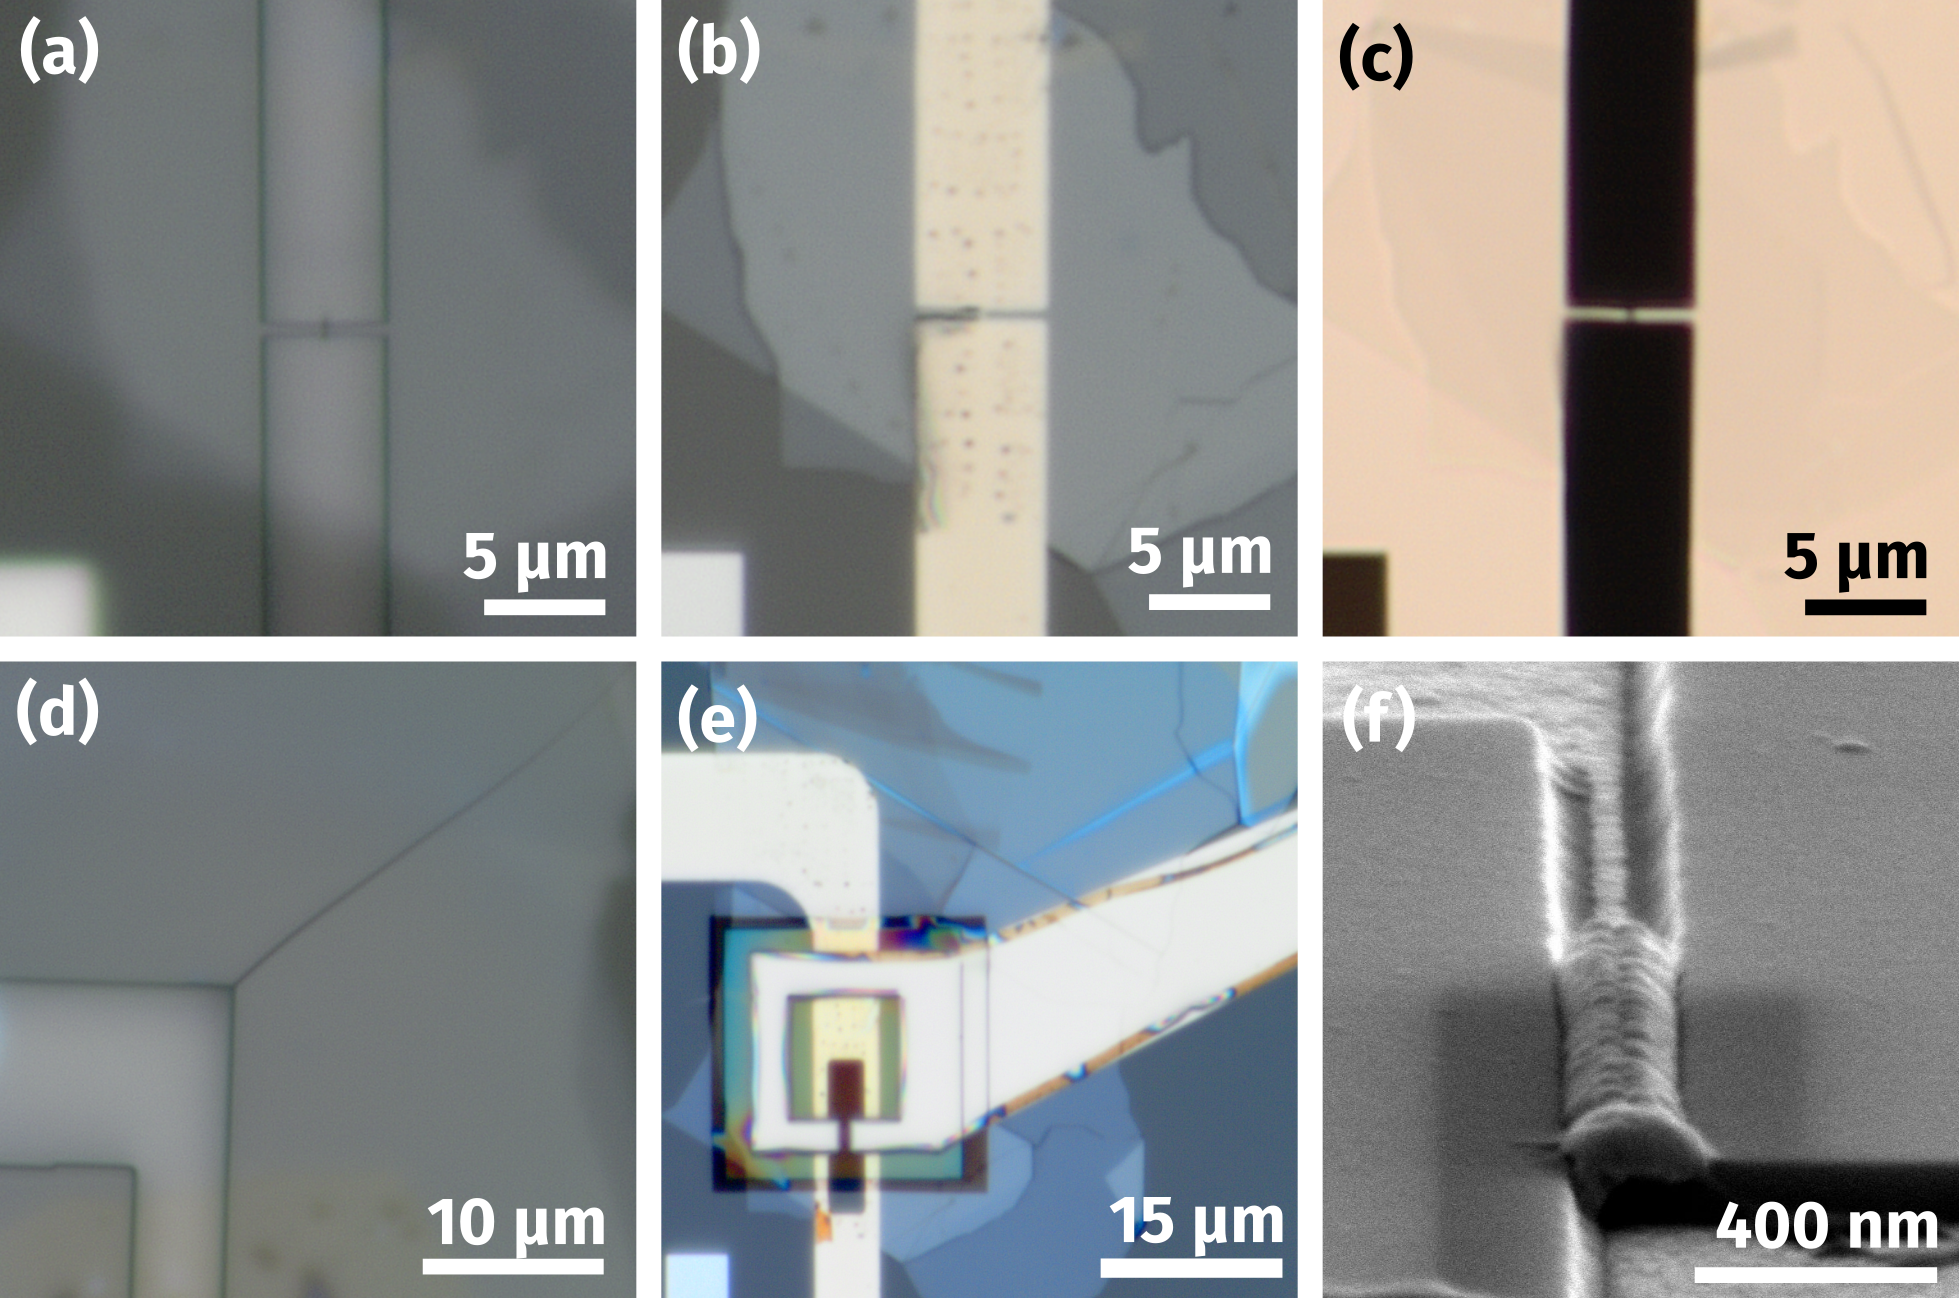
\includegraphics[]{{chapter-experimental-methods/figs-fabrication/fab-gJJ-challenges.svg}.png}
	\caption{
		% 
		\textbf{Challenges associated with gJJ fabrication.}
		% 
		\textbf{(a-c)} Due to the insulating nature of sapphire, ebeam patterning can lead to the substrate charging up and overexposing parts of the resist. 
		% 
		After developing \textbf{(a)}, dark spots in the resist in the gap center are due to developed resist due to charging effects.
		%
		\textbf{(b)} After etching and lift-off, the junction is shorted in the center and dog-ears are visible to the right side, standing up.
		% 
		\textbf{(c)} Illumination through the backside of the sapphire substrate reveals a nanobridge short.
		% 
		\textbf{(d)} Insufficient resist adhesion to the substrate and resist tension can lead to cracks originating at sharp bends and extending several tens of microns.
		%
		\textbf{(e)} Significant dog-ears after liftoff are visible as colored bands on top of the metal film of a top-gate extending over a graphene SQUID.
		% 
		\textbf{(f)} SEM image of two superconducting banks on sapphire, partially connected by two dog-ears across the gap.
	}
	\label{fig:fabgJJchallenges}
\end{figure}

\begin{figure}
	\centering
	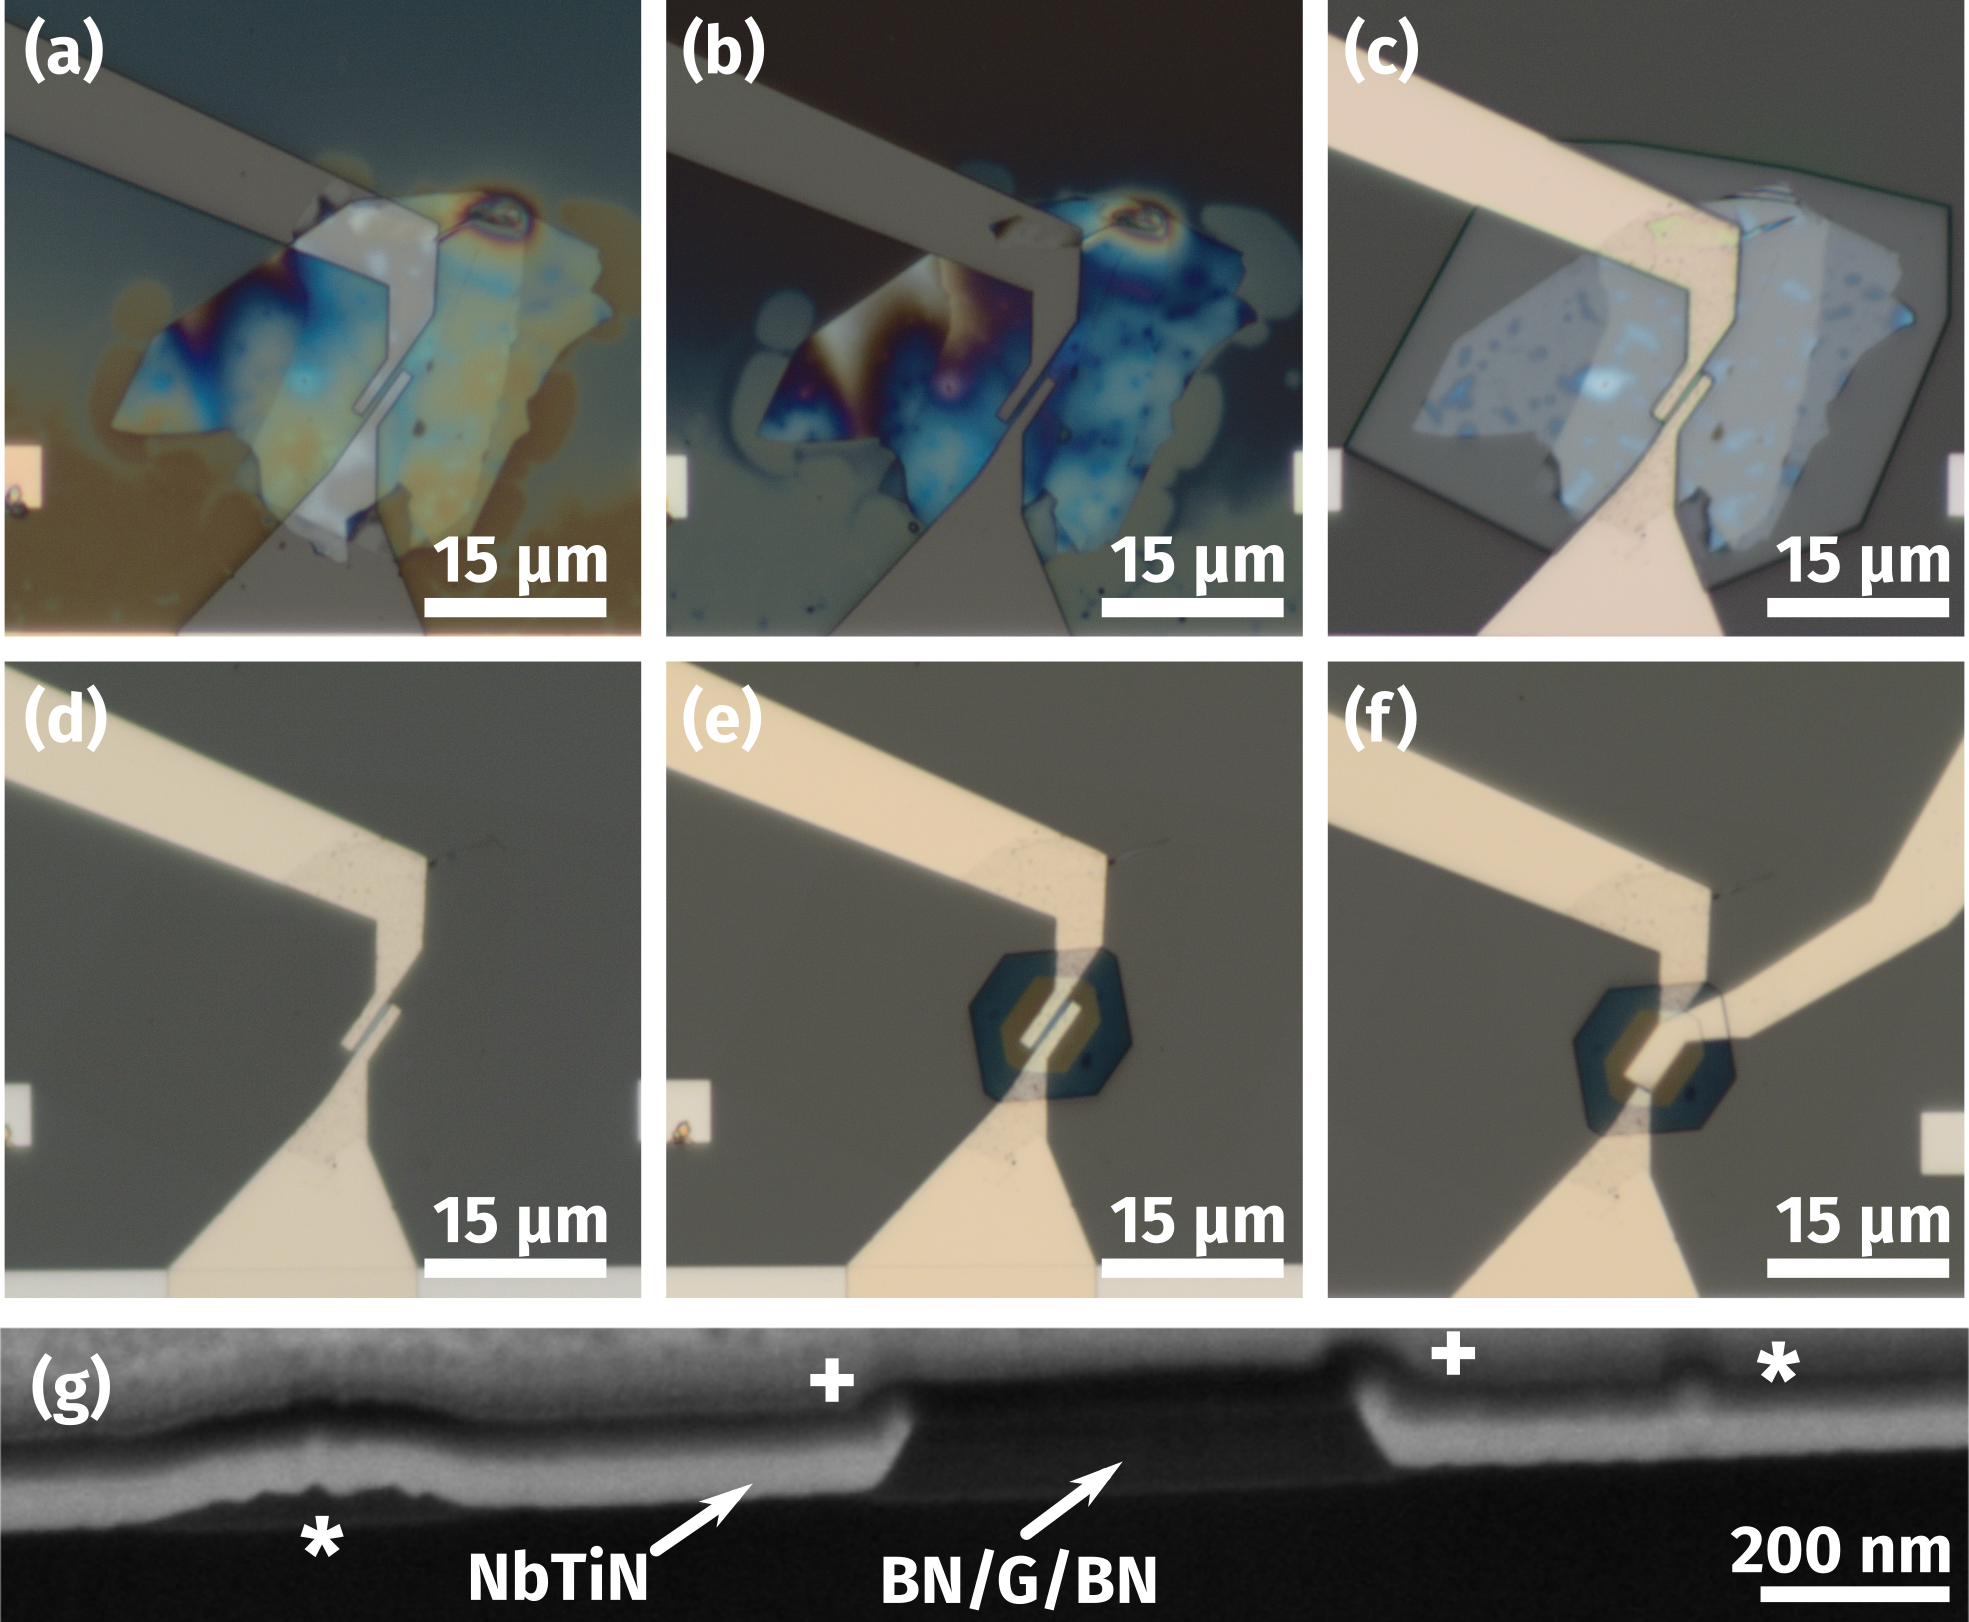
\includegraphics[]{{chapter-experimental-methods/figs-fabrication/fab-gJJ.svg}.png}
	\caption{
		% 
		\textbf{From stack to device: Fabrication of top-gated graphene Josephson junctions.}
		% 
		\textbf{(a)} BN-G-BN sandwich on sapphire substrate. The optical micrograph is loaded into a CAD program and aligned with respect to the prepatterned markers.
		% 
		After electron beam exposure and development, the areas to be metallized are open, while the rest of the substrate remains covered by the resist.
		% 
		\textbf{(b)} In order to make galvanic contacts to the graphene layer, the chip is placed in a \ce{CHF3 + O2} plasma, which dry-etches the BN layer.
		% 
		Careful etch-rate calibration is required to not under-etch for good contact to the graphene while not over-etching so that enough PMMA is left for successful liftoff.
		% 
		\textbf{(c)} Sample after metallization and lift-off, with etch mask for shaping the stack into the final shape.
		% 
		\textbf{(d)} Sample after patterning into rectangular shape.
		%
		Only the gJJ slab remains.
		%
		\textbf{(e)} Bilayer HSQ covering the stack and metal leads as an insulating gate dielectric.
		% 
		\textbf{(f)} Finalized sample with superconducting gate electrode extending over the entire Josephson junction.
		\textbf{(g)} Cross-sectional SEM of a gJJ resting on silicon, contacted by NbTiN.
		%
		Contact angles are approximately \SI{60}{\degree}.
		%
		Defects such as bubbles (*) and dog-ears (+) are visible.
		%
		Courtesy of Triantafyllia (Rose) Sermpeniadi/Conesa-Boj lab.
	}
	\label{fig:fabgJJ}
\end{figure}

\begin{table}
	\caption{
		\textbf{Fabrication of side-contacted top-gated graphene Josephson junctions.}
		%
		Note that after washing off Electra 92, the chip needs to be blow-dried before developing the PMMA.
		%
		Electra is not necessarly needed for the top-gate dielectric and gate metal.
	}
	\label{tab:fabgJJ}
\begin{tabularx}{\textwidth}{@{}cY@{}}
	\hline \hline
	\textbf{1.} & \textbf{Making NbTiN contacts using etch-fill} \\
	\hline
	Ebeam resist (1/2) & PMMA 495 A4, \SI{4000}{rpm}, bake \SI{10}{\minute} at \SI{185}{\celsius} \\
	Ebeam resist (2/2) & PMMA 950 A3, \SI{4000}{rpm}, bake \SI{10}{\minute} at \SI{185}{\celsius}. \\
	%\hline
	Conductive resist & Electra 92, \SI{2000}{rpm}, bake \SI{90}{\second} at \SI{80}{\celsius}. \\
	Ebeam patterning & \SI{1000}{\micro\coulomb\per\centi\meter\squared} + PEC \\
	%\hline
	Wash off Electra 92 & Rinse in water for \SIrange{30}{60}{\second}. \\
	Development & MIBK:IPA (1:3) for \SI{90}{\second}, IPA \SI{30}{\second}. \\
	%\hline
	Dry etching & \ce{CHF3 + O2} \SI{40}{sccm}+\SI{4}{sccm} @ \SI{60}{\watt}, \SI{80}{\micro\bar} for \SI{1}{\minute} (etch rate roughly \SI{60}{\nano\meter\per\minute}) \\
	%\hline
	Metal deposition & \SI{5}{\nano\meter} NbTi and \SIrange{60}{70}{\nano\meter} NbTiN \\
	%\hline
	Liftoff & hot PRS~3000 @ \SI{88}{\celsius} for a few hours, rinsing in IPA \\
	\hline
	\textbf{2.} & \textbf{Shaping the device:} \\
	\hline
	& Same resist, patterning and etching as for making the contacts, but with lower etch pressure (\SI{50}{\micro\bar}) and no metal deposition. \\
	\hline
	\textbf{3.} & \textbf{Top-gate dielectric} \\
	\hline
	Ebeam resist & concentrated HSQ, \SI{8000}{rpm}, bake \SI{10}{\minute} at \SI{90}{\celsius} in an oven. \\
	%\hline
	Ebeam patterning & \SI{1000}{\micro\coulomb\per\centi\meter\squared}. \\
	%\hline
	Development & MF322 for \SI{1}{\minute}, MF322:\ce{H2O} (1:9) for \SI{15}{\second}, \ce{H2O} for \SI{15}{\second}. \\
	%\hline
	& Repeat this process once. \\
	\hline 
	\textbf{4.} & \textbf{Top-gate metal: } \\
	\hline
	& Same steps as for making the contacts, but no etching and with metal thickness of \SIrange{80}{120}{\nano\meter}. \\
	\hline \hline
\end{tabularx}
\end{table}


\clearpage
\subsection{Fabrication of DC bias cavities}\label{sec:fabRF}

The process for fabricating DC bias cavities consists of three main steps:
\begin{itemize}
	\item Deposit and pattern base layer (CPW, ground plane, shunt bottom part)
	\item Deposit and pattern shunt dielectric
	\item Deposit and pattern shunt top plate
\end{itemize}
%
For best fabrication results, a mono-layer of HMDS should be applied before every resist spinning, as described in Sec.~\ref{sec:fabgJJ}.
%
The use of Electra 92 for devices on sapphire is not strictly necessary due to the large feature size and the conducing metal base layer, but still recommended.

Care needs to be taken to ensure that there are no shorts in the shunt dielecric layer.
%
Since the dielectric deposition using PECVD does not necessarily provide complete step coverage, the dielectric layer should be at least \SI{30}{\percent} thicker than the base layer.
%
We found this to be problematic when patterning the base layer using dry etching on silicon substrates because the dry-etch process can cut deep into the silicon substrate, increasing the step height to be covered by the dielectric.
%
In this case, depositing a dielectric fill layer in the gaps slightly extending above the step edges, resulted in reliable device yield.

Instead of wet-etching the shunt capacitor dielectric, dry-etching using a \ce{CHF3 + O2} plasma at \SI{60}{\watt} power and base pressure of \SI{50}{\micro\bar} yielded comparable results.
%
However, the combination of plasma etching with negative ebeam resist often resulted in teflonization of the latter, severely complicating resist stripping afterwards.
%
This can be avoided by either in-situ \ce{O2} ashing, or by applying a thin PMMA layer below the negative ebeam resist, which can be stripped off the sample much easier.
%
From a safety perspective, the plasma etch process is to be preferred over the use of BOE due to the much lower risk to the operator.
%
Additionally, even though wet-etching seems to be a cleaner process compared to dry-etching, the obtained internal quality factors of samples fabricated using BOE did not consistently surpass those of dry-etched devices.

\begin{figure}
	\centering
	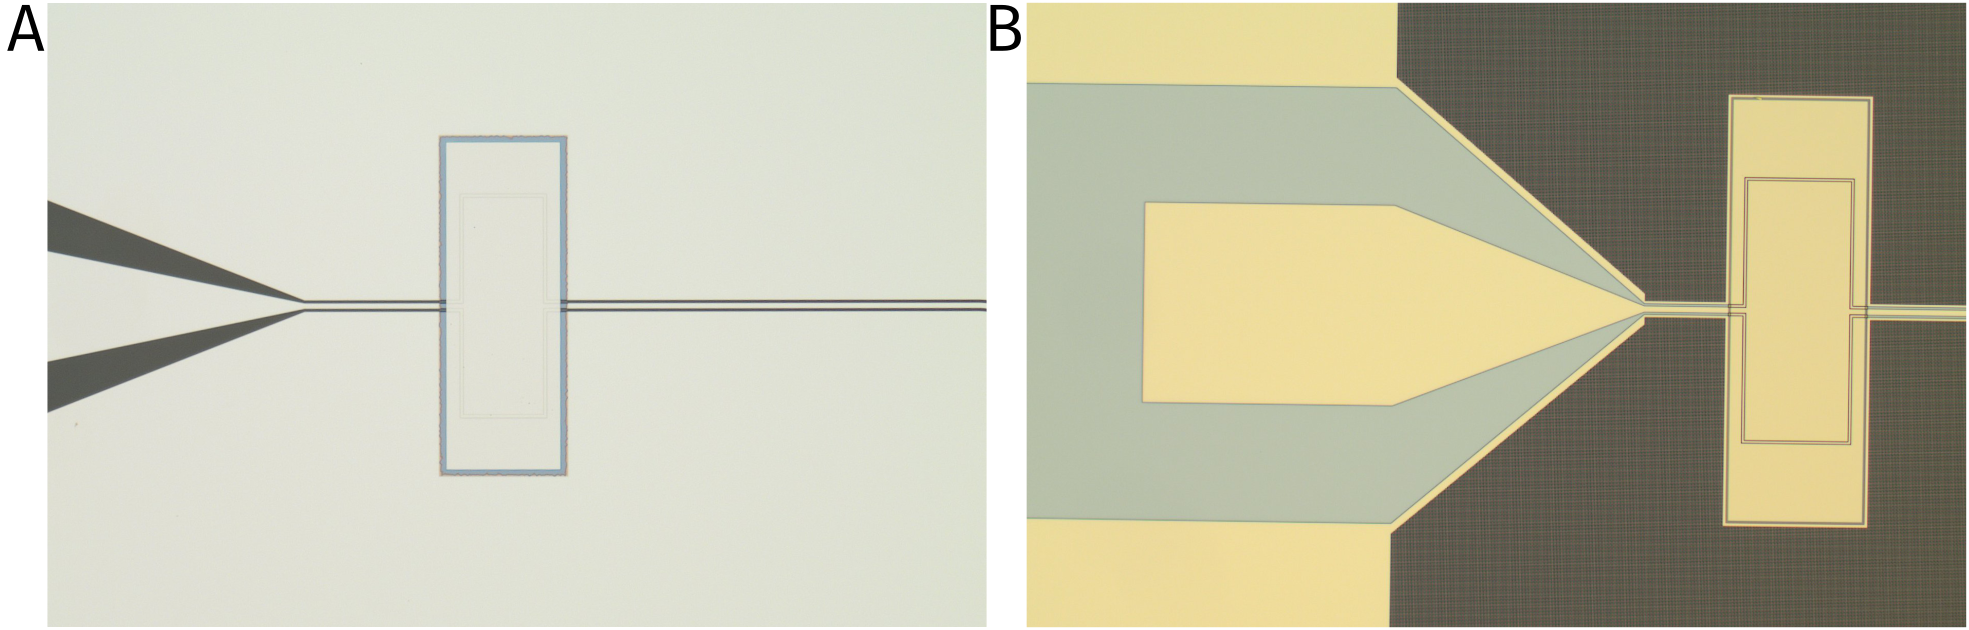
\includegraphics{{chapter-experimental-methods/figs-fabrication/fab-shunt-bias.svg}.png}
	\caption{
		\textbf{Finished current-bias microwave cavities.}
		% 
		\textbf{(a)} DC bias cavity on sapphire with MoRe base and top layer and \ce{Si3N4} capacitor dielectric.
		%
		\textbf{(b)} Device on silicon with aluminum base and top layer and Si capacitor dielectric.
		%
		\textbf{(c)} Device on silicon with NbTiN base and top layer and \ce{Si3N4} capacitor dielectric.
		%
		The third device features holes in the ground plane in an effort to reduce magnetic flux focusing and trap vortices.
	}
	\label{fig:biascavityfab}
\end{figure}

%\noindent
\begin{table}
	\caption{
		\textbf{Fabrication of DC-bias superconducting microwave cavities.}
		%
		This is the recipe for the circuits in Chapters~\ref{chap:gJJ} and \ref{chap:gJJ-CPR}.
	}
	\label{tab:fabRF}
	\begin{tabularx}{\textwidth}{@{}cY@{}}
		\hline \hline
		\textbf{1.} & \textbf{Deposit and pattern MoRe base layer} \\
		\hline 
		Metal deposition & \SI{60}{\nano\meter} MoRe, \SI{100}{\watt}, \SI{60}{sccm} Argon flow. \\
		%\hline
		Ebeam resist & AR-P 6200.13 (CSAR), \SI{4000}{rpm}, bake \SI{3}{\minute} at \SI{155}{\celsius}. \\
		%\hline
		Ebeam patterning & \SI{300}{\micro\coulomb\per\centi\meter\squared}. \\
		%\hline
		Development & Pentylacetate for \SI{60}{\second}, MIBK:IPA (1:1) for \SI{30}{\second}, IPA for \SI{15}{\second}. \\
		%\hline
		Dry etching & \ce{SF6 + He} \SI{12.5}{sccm}+\SI{10}{sccm} @ \SI{50}{\watt}, \SI{10}{\micro\bar} \\
		%\hline
		Liftoff & hot PRS~3000 @ \SI{88}{\celsius} for a few hours, rinsing in IPA \\
		\hline
		
		\textbf{2.} & \textbf{Deposit and pattern dielectric layer for shunt capacitor} \\
		\hline 
		Dielectric deposition & PECVD \SI{70}{\nano\meter} of \ce{Si3N4} @ \SI{300}{\celsius}. \\
		%\hline
		Ebeam resist & AR-N 7700.18, \SI{3000}{rpm}, bake \SI{1}{\minute} at \SI{90}{\celsius}. \\
		%\hline
		Ebeam patterning & \SI{210}{\micro\coulomb\per\centi\meter\squared}. \\
		%\hline
		Development & MF321 for \SI{60}{\second}, MF321:\ce{H2O} (1:10) for \SI{15}{\second} (twice), \ce{H2O} for \SI{15}{\second}. \\
		%\hline
		Wet etching & BOE \SI{1}{\minute} \\
		%\hline
		Strip resist & hot PRS~3000 @ \SI{88}{\celsius} for a few hours, rinsing in IPA \\
		\hline
		
		\textbf{3.} & \textbf{Deposit top metal plate of shunt capacitor} \\
		\hline 
		Ebeam resist (1/2) & PMMA 495 A4, \SI{4000}{rpm}, bake \SI{10}{\minute} at \SI{185}{\celsius}. \\
		%\hline
		Ebeam resist (2/2) & PMMA 950 A3, \SI{4000}{rpm}, bake \SI{10}{\minute} at \SI{185}{\celsius}. \\
		%\hline
		Ebeam patterning & \SI{1400}{\micro\coulomb\per\centi\meter\squared}. \\
		%\hline
		Development & MIBK:IPA (1:3) for \SI{90}{\second}+ IPA \SI{30}{\second}. \\
		%\hline
		Metal deposition & \SI{100}{\nano\meter} MoRe as described above. \\
		%\hline
		Lift-off & hot PRS~3000 @ \SI{88}{\celsius} for a few hours, rinsing in IPA \\
		\hline\hline
	\end{tabularx}
\end{table}

The RF circuits in Chapters~\ref{chap:gJJ} and \ref{chap:gJJ-CPR} are fabricated as listed in Tab~\ref{tab:fabRF}, while the one in Chapter~\ref{chap:currentdetection} used Al:Si as superconducting layer and silicon as substrate and dielectric layer.
%
In terms of internal quality factor $Q_\text{i}=\omega_0/\kappa_\text{i}$, the best devices with sapphire substrate and MoRe base layer showed $Q_\text{i}\approx\num{41e3}$, while DC bias cavities out of aluminum on silicon substrates and shunt dielectric had $Q_\text{i}\approx\num{29e3}$.
%
While not used for further measurements in this thesis, the reproducibly highest internal quality factors were achieved with sputter-deposited NbTiN on silicon after intensive wafer cleaning by our collaborators at \textit{SRON}~\cite{thoenSuperconductingNbTinThin2017}, and \ce{Si3N4} as dielectric with BOE patterning.
%
Figure~\ref{fig:s11NbTiN} shows the resulting reflection measurement of the best measured sample (cf. Fig.~\ref{fig:biascavityfab}(c)), with an internal quality factor $Q_\text{i}\approx\num{82439}$.
%
In comparison, $\lambda/4$ side-coupled resonators from the same wafer fabricated in a single step exhibited internal quality factors exceeding 1 million.

Even higher device quality could be achieved with a low-loss dielectric such as \ce{Al2O3} and a more local deposition:
%
We speculate that depositing dielectric on the entire chip area might degrade the film quality by damaging the superconducting layer in areas where voltage fluctuations are non-negligible, thus introducing defects such as two-level systems which can absorb radiation and lead to internal losses.
%
Additionally, device patterning with dry-etching can physically roughen the superconducting base layer.
%
Even wet-etching, such as with BOE, can leave behind defects.
%
For example, we observed that ALD-deposited \ce{Al2O3} left micron-sized flakes on the chip, that could not entirely get dissolved in BOE.
%
As an alternative, we propose local deposition by liftoff, as can be done with low-temperature PECVD or ALD.
%
This could protect the surrounding circuitry and potentially reduce internal circuit losses.

\begin{figure}
	\centering
	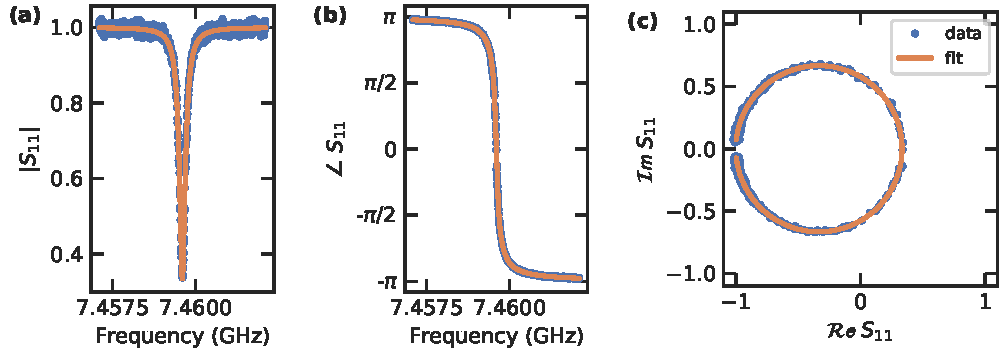
\includegraphics[width=\linewidth]{chapter-experimental-methods/figs-fabrication/data_gJJ_ref_Qint}
	\caption{
		\textbf{Reflection coefficient of the best fabricated DC bias cavity.}
		%
		Data (blue points) and fit (orange line) to the absolute value \textbf{(a)}, phase \textbf{(b)} and real and imaginary parts \textbf{(c)} of the reflection coefficient of a DC bias cavity with NbTiN base layer on silicon, the device in Fig.~\ref{fig:biascavityfab}(c).
		%
		The internal and external quality factors are $Q_\text{i}\approx\num{82439}$ and $Q_\text{i}\approx\num{41209}$.
	}
	\label{fig:s11NbTiN}
\end{figure}

\clearpage
\section{DNA-like oxidation of MoRe thin films}
\label{sec:more}

During his times as postdoc at TU Delft, my supervisor Gary Steele found that the superconducting alloy molybdenum-rhenium was the only suitable superconductor to sustain the growth conditions of carbon nanotubes.
Moreover, the work function of MoRe matches that of graphene quite close, which was why its use was further pushed in the field of hybrid carbon-superconductor devices.
However, it was often overlooked that devices made from MoRe began exhibiting peculiar "spots" visible under an optical microscope after a few days.

We found that there were small "crystallites" growing on the surface of sputtered MoRe films, regardless of wafer substrate and film thickness.
Growth of these structures seems to be forming by seed-growth of small islands less than \SI{1x1}{\micro\meter} in size (cf. Figs.~\ref{fig:MoreDNA}C,D) which would then diffuse on the surface and cluster together in DNA-like strands (cf. Fig.~\ref{fig:MoreDNA}B).
This growth mechanism covers the entire film surface with small islands, lumping together into bigger structures, as depicted in Fig.~\ref{fig:MoreDNA}A.
Remarkably, some of the largest crystals grew even higher in the third dimension than the original MoRe film thickness.

Analzying the atomic composition of these crystallites using EDX peak intensity lead us to believe that the they are mainly composed of rhenium oxide, judging from the reduced molybdenum EDX peak intensity compared to the one of rhenium at these spots, cf. Fig~\ref{fig:moreedx}.
The signal originating from the silicon peak (c) is expected to be weaker at the crystal location since due to less X-ray radiation can reach the detector because of the increase in thickness.
In contrast to the reduced silicon and molybdenum peaks, the oxygen and rhenium signals are stronger at the crystal location, strongly hinting at some kind of rhenium oxide.

Further, quantitative compositional analysis could not be performed because the oxygen signal is very close to the zero loss peak and the rhenium and molybdenum content of the surface layer would have some contribution of the bulk below.
Our observation contrasts the one made on thin and bulk MoRe structures in literature, where \ce{MoO3} and \ce{MoO2} were found to be the dominant oxide~\cite{seleznevDepositionCharacterizationFewnanometersthick2008b,gotzCosputteredMoReThin2016}.
To the best of our knowledge, there is however no literature on the observed ReO crystallites.

While the superconducting critical temperature of large structures of this film seemed to be unaffected by the growth, these structures can severely degrade the high-frequency response of superconducting circuits such as resonators or qubits, as dielectric losses can be one of the main reasons for qubit decoherence~\cite{lisenfeldElectricFieldSpectroscopy2019}.
Moreover, since the crystallites physically move about on the film surface, they might interfere with any patterned structures, leading to unintended defects in or even damage the electrical wiring.
We found that a \SI{60}{\second} dip of MoRe films in strong oxidizing agents, such as MF321 or BOE, was enough to wash off these crystallites as longs as they were still in the seed phase, and the density of big clusters was low.
This corresponds to a storage time below three days in ambient conditions.
Crystal seeding sets in almost immediately and is clearly visible under an optical microscope at 5x magnification after one day. 
The crystal growth can be slowed down significantly, but not completely suppressed, if films are stored in dry boxes with constant nitrogen flow.
We estimate that one day in ambient conditions has the same effect as two weeks in nitrogen atmosphere.

Since the devices studied in this thesis did not require MoRe per se, we chose to abandon this superconducting alloy after thorough investigation, and switched to NbTiN or aluminum, depending on the specific circuit requirements.

\begin{figure}
	\centering
	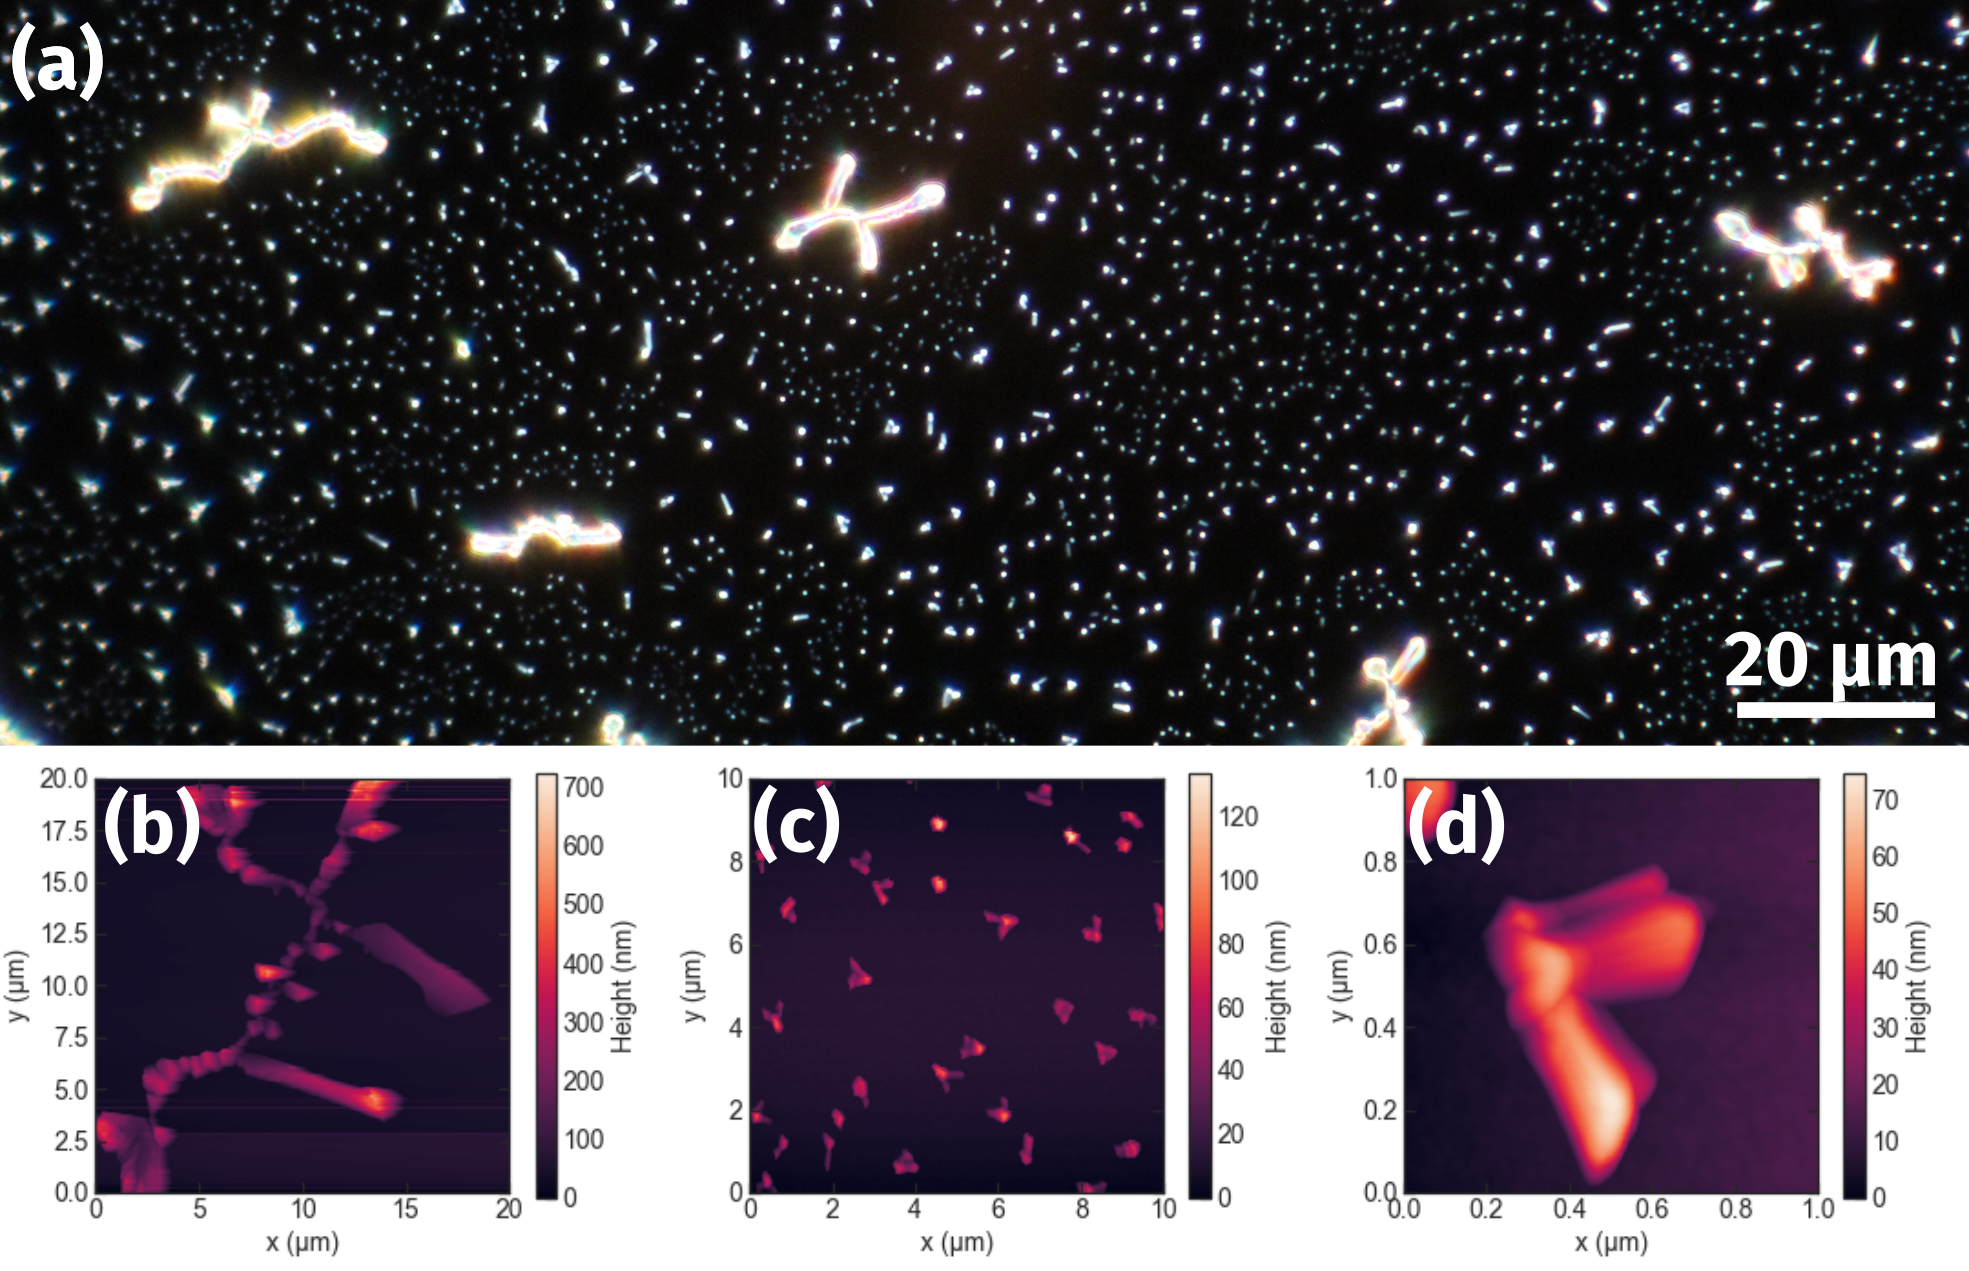
\includegraphics[]{{chapter-experimental-methods/figs-fabrication/MoreDNA.svg}.png}
	\caption{
		\textbf{DNA-like oxidation of MoRe thin films.}
		\textbf{A,} Optical image of MoRe film under and dark field after two weeks in ambient conditions.
		Scale bar \SI{25}{\micro\meter}.
		\textbf{B-D,} AFM images of several locations and types on the film:
		Small individual crystallites (B) serve as seed islands on the film surface (C), which then agglomerate into DNA-like strands (D), covering the entire film surface (A).
		MoRe film thickness \SI{100}{\nano\meter}.
	}
	\label{fig:MoreDNA}
\end{figure}

\begin{figure}
	\centering
	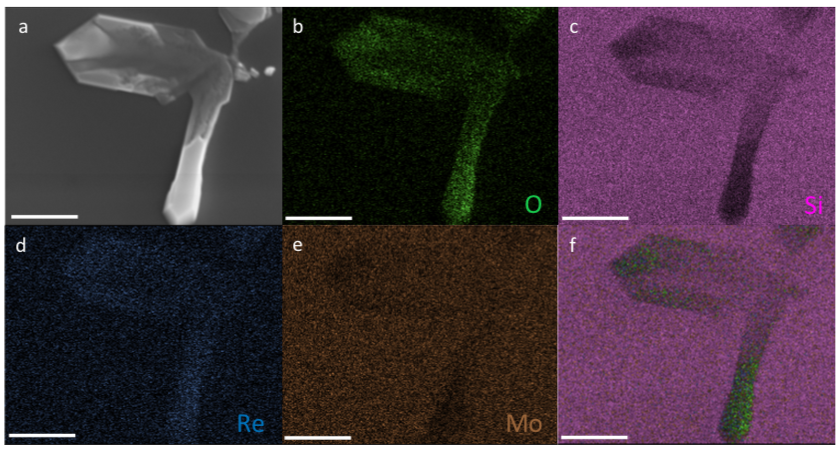
\includegraphics[width=\linewidth]{chapter-experimental-methods/figs-fabrication/pics/MoRe_EDX}
	\caption{
	\textbf{EDX spectra of MoRe crystallites on silicon substrate.}
	\textbf{a,} SEM image of a region in the MoRe layer.
	\textbf{b-e,} EDX elemental maps of O, Si, Re and Mo respectively.
	\textbf{f,} Superposition of the \textbf{b-e} elemental maps.
	All scale bars \SI{2}{\micro\meter}.
	Courtesy of Dr. Miguel Tinoco-Rivas/Conesa-Boj lab, TU Delft.
	}
	\label{fig:moreedx}
\end{figure}

\section{Measurement setup}

\subsection{Device post-processing and packaging}\label{sec:fab-packaging}

Once device fabrication is finished, the sample has to be mounted on a chip carrier and contacted, so we can connect it to our measurement electronics.
% 
Our microwave PCBs are made for \SI{10x10}{\milli\meter} chips.
%
However, in order to better hold on to the chips during fabrication and to enhance the fabrication yield, samples are usually fabricated on larger substrates:
% 
The current bias cavities for the graphene devices presented in Chapters~\ref{chap:gJJ} and \ref{chap:gJJ-CPR} were processed on a \SI{2}{inch} wafer, and the cavities based on aluminum in Chapter~\ref{chap:currentdetection} on \SI{15x15}{\milli\meter} chips.

We dice the chips into the correct dimensions in the very last step, using a \textit{Disco dicer DAD 3220} from \textit{Disco Hi-Tec Europe GmbH}.
% 
To protect the chip from dust during sawing, we spincoat photoresist\footnote{HPR504, \SI{4000}{rpm}, bake \SI{60}{\second} at \SI{100}{\celsius}, approximately \SI{1.2}{\micro\meter} thick} on the chip before dicing.
% 
Good resist-substrate adhesion is important because the water jet used to cool the blade can wash off the resist during dicing otherwise, potentially ruining weeks of delicate work in the cleanroom.
% 
Use of HMDS, or letting the resist sit on the chip to be diced for \SI{1}{\minute} prior to spinning, is therefore strongly recommended.

The silicon chips were diced using a standard NBC blade at \SI{3000}{rpm} and a feed speed of \SI{5}{\milli\meter\per\second}, while for dicing sapphire we used a special diamond blade at \SI{2000}{rpm} and \SI{2}{\milli\meter\per\second}.
% 
For the devices presented in this thesis, we placed the diced chips in teflon holders inside beakers filled with PRS3000, heated the solution to \SI{80}{\celsius} and subsequently put the beaker into an ultrasound bath at maximum power.
% 
After \SI{5}{\minute}, the resist has then come off the sample, and we passed the chip through a series of PRS3000 and IPA baths to wash off any remains, and blow-dried using nitrogen.


For electrical measurements, the chips are wirebonded to PCBs that are mounted on copper boxes, cf. Fig.~\ref{fig:packaging}.
%
The bottom part of the first generation copper boxes, on which the chip rests, had a simple flat base.
%
However, we noticed that this lead to cross-talk of devices across the entire chip, presumably due to electromagnetic box modes between substrate and copper base.
%
To mitigate this spurious coupling, we removed most of the copper base to leave only two thin rails behind, to which the chips are glued with GE low temperature varnish.
% 
Wirebonding is done using a \textit{Westbond 4000 "E"} system from \textit{West•Bond Inc.} with bond wires from an AlSi alloy (\SI{99}{\percent}-\SI{1}{\percent}).
% 
To ensure good thermalization and electrical contact, we usually used three to four bonds for each bond pad, and as many bonds as would fit on the ground planes.
% 
An example of one of our devices that is mounted and wirebonded in a PCB, ready for measurement can be seen in Fig.~\ref{fig:packaging}.
% 
The connectors to go from the PCB to the outside world are straight plug semi-detent SMP connectors\footnote{19S102-40ML5 straight plug PCB, from \textit{Rosenberger Hochfrequenztechnik GmbH \& Co. KG}}.


\begin{figure}
	\centering
	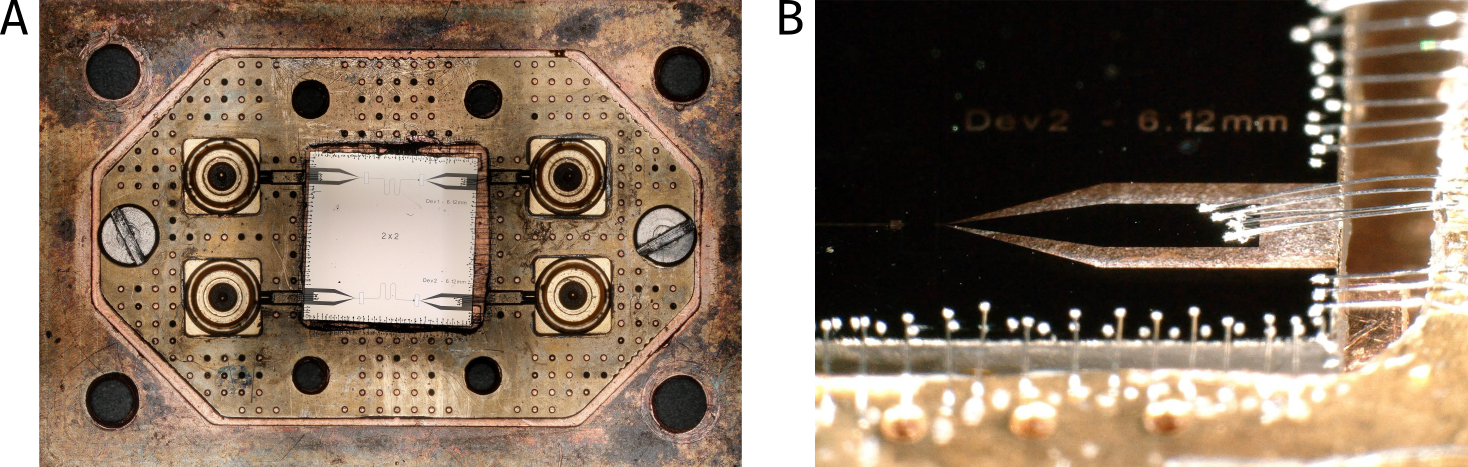
\includegraphics{{chapter-experimental-methods/figs-packaging/packaging.svg}.png}
	\caption{
		\textbf{Device packaging for electrical measurements.}
		% 
		\textbf{(a)} The \SI{10x10}{\milli\meter} chip is mounted and wirebonded to a PCB, that is screwed onto a copper base.
		% 
		The four small holes around the chip are used to screw on a small copper lid, covering the chip.
		% 
		The four big holes at the edge of the copper base are used for mounting the chip in a cryostat, and to hold the top cover in place.
		% 
		Connectors for connecting the PCB to the outside world are surface mount SMP plugs.
		% 
		\textbf{(b)} Close-up of the bottom-right chip area, taken with ring illumination.
		% 
		The substrate is sapphire, hence the chip transparency.
		% 
		In the bottom right corner, one of the copper rails on which the chip sits is visible.
		%
		\textbf{(c)} The individual parts of our sample holder (clockwise):
		%
		PCB for \SI{10x10}{\milli\meter} chips, copper base with rails to mount chip and PCB, small cover, large lid.
		%
		\textbf{(d)} Sample enclosed and mounted in the bottom-loading puck of a \textit{Triton} dilution fridge.
		%
	}
	\label{fig:packaging}
\end{figure}

\subsection{Filtering and attenuation}

\subsubsection{Low frequency interference}

Current and voltage fluctuations originating from room temperature electronics can carry the typical \SI{50}{\hertz} interference (also dubbed \textit{mains hum}), along with other, high-frequency, components.
%
In our lab, we suppress the mains hum by using battery-powered DC electronics for probing and biasing our circuits, the IVVI rack, made at \textit{DEMO}\footnote{Dienst Elektronische en Mechanische Ontwikkeling, \url{https://www.tudelft.nl/demo/}} of TU Delft.
%
The IVVI is controlled via an optical fiber connected to the measurement PCs.

Still, as shown in the Supplementary Material of Chapter~\ref{chap:currentdetection}, to properly suppress the mains hum, battery and mains powered equipment needs to be physically separated from each other.
%
This requires separate grounds between the two, DC blocks for inner and outer conductor attached to all high-frequency lines, as well as placing the IVVI and mains powered equipment on separate racks.

\subsubsection{Thermal excitation}

Thermal excitation can contribute to quasiparticles in the superconductor, meaning introducing a population of unpaired electrons, compared to the lossless Cooper pairs.
%
Table~\ref{tab:fthermal} lists the thermal energies and frequencies corresponding to typical temperatures in our setups.
%
The origin of these excitations in the so-called Johnson-Nyquist noise due to the thermally activated motion of charge carriers in conductors, regardless of applied voltage~\cite{johnsonThermalAgitationElectricity1928,nyquistThermalAgitationElectric1928}.

\begin{table}
	\caption{\textbf{Frequencies and energies of thermal noise.}}
	\label{tab:fthermal}
\begin{tabular}{ccc}
	\hline \hline
	Temperature & Thermal frequency & Thermal energy \\ 
	\hline 
	\SI{300}{\kelvin} & \SI{6.25}{\tera\hertz} & \SI{25.9}{\milli\electronvolt} \\ 
	% \hline 
	\SI{50}{\kelvin} & \SI{1.04}{\tera\hertz} & \SI{4.3}{\milli\electronvolt} \\ 
	% \hline 
	\SI{4}{\kelvin} & \SI{83.3}{\giga\hertz} & \SI{345}{\micro\electronvolt} \\ 
	% \hline 
	\SI{1}{\kelvin} & \SI{20}{\giga\hertz} & \SI{86.2}{\micro\electronvolt} \\ 
	\SI{100}{\milli\kelvin} & \SI{2}{\giga\hertz} & \SI{8.62}{\micro\electronvolt} \\ 
	% \hline 
	\SI{10}{\milli\kelvin} & \SI{208}{\mega\hertz} & \SI{862}{\nano\electronvolt} \\ 
	\hline \hline
\end{tabular}
\end{table}

In order to neglect the influence of thermal effects on our circuits and for the superconductor to be in its thermal ground state, it is necessary to operate the devices at temperatures $T \ll T_c$.
%
Since the superconducting gap voltages of \ce{NbTiN}, \ce{MoRe} and \ce{Al} are \SI{2.3}{\milli\electronvolt}, \SI{1.5}{\milli\electronvolt} and \SI{183}{\micro\electronvolt}, respectively, our experiments require access to the sub-Kelvin regime which is enabled by using dilution refrigerators.
%
However, even with the devices mounted to the base plate of dilution refridgerators (the devices in Chapters~\ref{chap:gJJ} and \ref{chap:gJJ-CPR} in a \textit{Triton 200} from \textit{Oxford Instruments}, the one in Chapter~\ref{chap:currentdetection} in a \textit{LD-400} from \textit{Bluefors}), they still experience some active heat load due to the wiring connecting the sample to the room temperature electronics.
%
This way, thermal noise can couple into the devices.
%
It is therefore vital to suppress this noise by means of signal attenuation before reaching the sample, while not sacrificing too much signal-to-noise ratio.



While attenuating the input lines as much as possible seems to be a good idea at first, this is not necessary because the physical temperature of the lowest fridge stage, in our experiments the base temperature of $T_{\rm MXC}\approx\SI{15}{\milli\kelvin}$, places a lower bound on the sample temperature, and therefore on the required lowest noise temperature.
%
Additionally, due to low electron-phonon coupling at low temperatures, the electrons in the device most likely have a slightly larger temperature than the fridge itself, as cooling becomes inefficient at these temperatures~\cite{giazottoOpportunitiesMesoscopicsThermometry2006}.
%
Cooling below the fridge temperature is possible, but requires nuclear refrigeration in combination with further attenuation and low electron-phonon coupling~\cite{sarsby500MicrokelvinNanoelectronics2020}.
%

Since we will be probing our devices both at DC and with \si{\giga\hertz} frequencies, both low and high frequency lines need to be attenuated separately.
%
Our DC lines are attenuated using home-made two-stage RC and copper powder filters (see Appendix \ref{app:copperpowder} for details).
%
The RC filters have a cutoff frequency $f_{\SI{3}{\decibel}}\approx\SI{30}{\kilo\hertz}$ and suppress higher frequencies up to \SI{20}{\mega\hertz}.
%
Above this range, radiation starts to leak through again, due to stray capacitance of the filter resistors and parasitic inductance of the capacitors, cf. Fig.~\ref{fig:filterDC}(a,b).
%
As shown in Fig.~\ref{fig:filterDC}(b), a two-stage filter has a higher slope, \SI{-40}{dB/decade} compared to \SI{-20}{dB/decade}, while exhibiting only a slightly lower cut-off frequency.
%
The radiation leaking through calls for additional, very high-frequency lowpass filters.
%
We use home-made copper powder filters for this purpose, cf. Fig.~\ref{fig:filterDC}(c,d).
%
These consist of a long PCB trace encased in a copper box, which is filled with copper powder and epoxy, essentially forming a very long and lossy transmission line with very low resistance, suppressing frequencies above a few \SI{100}{\mega\hertz}, as shown in Fig.~\ref{fig:filterDC}(a).

\begin{figure}
	\centering
	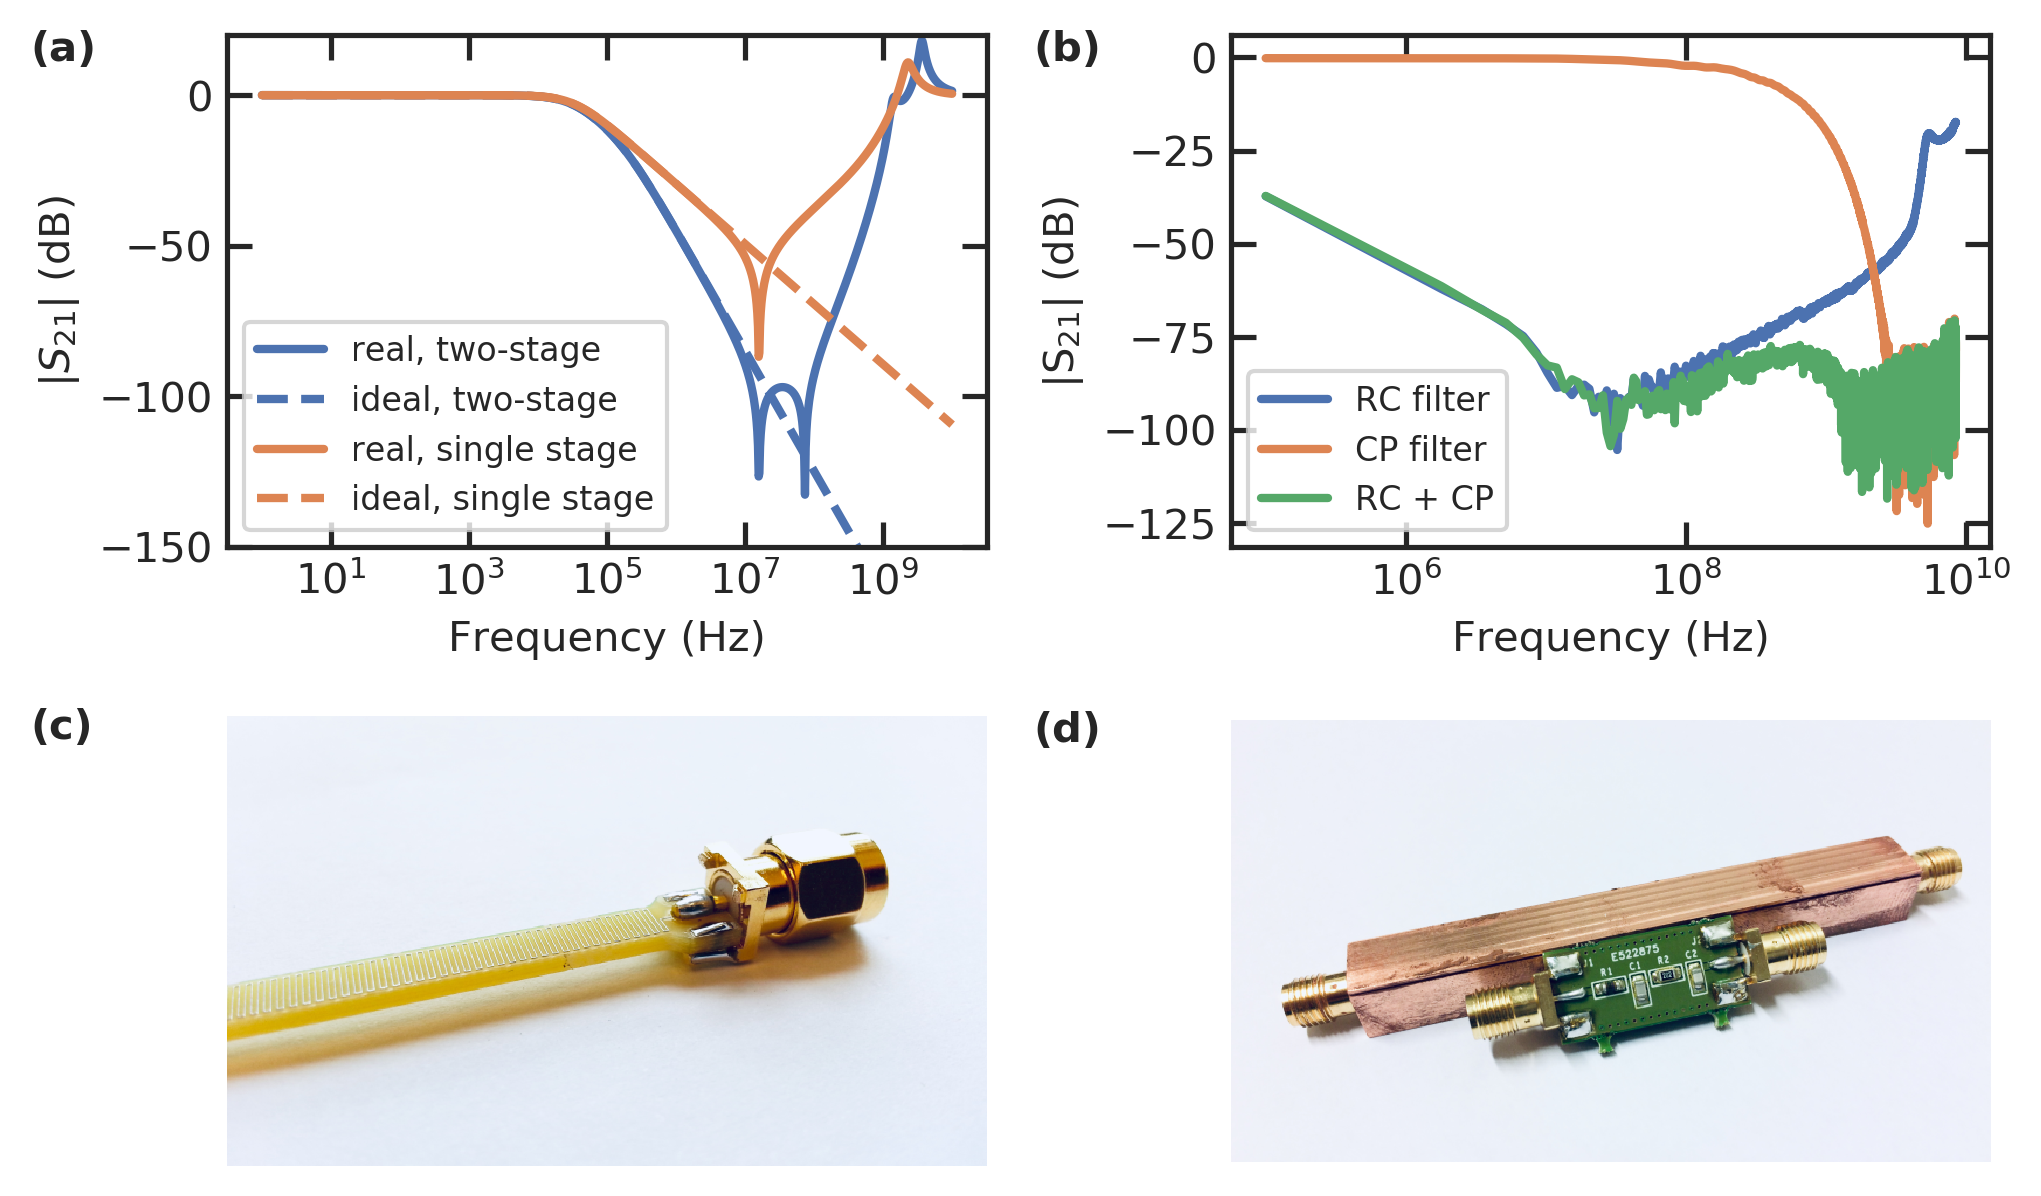
\includegraphics[width=\textwidth]{{chapter-experimental-methods/figs-setup/filterplots/DC_filters}.png}
	\caption{
		\textbf{Electronic noise reduction using low-pass filters.}
		%
		\textbf{(a)} Measured transfer function of combinations of two-stage RC lowpass and copper powder filters.
		%
		Parasitic inductance and capacitances in the RC filter allow radiation to leak through at higher frequencies, which can be suppressed using copper powder filters.
		%
		\textbf{(b)} Simulated transfer function of single (orange) and two-stage (blue) RC low-pass filters.
		%
		Dashed: ideal filter characteristic, solid: realistic behavior with stray capacitance and inductance.
		%
		\textbf{(c)} Copper powder filter PCB with connector, without enclosure.
		%
		The PCB trace is approximately \SI{50}{\centi\meter} long.
		%
		\textbf{(d)} Photograph of a two-stage RC filter of SMD 0812 elements and a fully assembled copper powder filter.
	}
	\label{fig:filterDC}
\end{figure}

We can estimate the effect of attenuation on the electron noise temperature~\cite{krinnerEngineeringCryogenicSetups2019}.
%
With the Bose-Einstein distribution
\begin{align}
n_{\rm BE}(f,T)=\frac{1}{e^{hf/k_B T}-1}\label{eq:nBE}
\end{align}
we can calculate the photon flux at frequency $f$ due to thermal noise coming from $T_1$ transmitted through a bath at $T_2$ with transmission $\tau$ with the rate equation
\begin{align}
n_{\rm ph}(f,T_1,T_2,\tau)=\tau n_{\rm BE}(f,T_1)+(1-\tau)n_{\rm BE}(f,T_2)\label{eq:nphot}
\end{align}
The noise temperature of the corresponding photon flux is then
\begin{align}
T_{n}=\frac{hf}{k_B\ln\left(\frac{n_{\rm ph}+1}{n_{\rm ph}}\right)}
\label{eq:Tnoise}
\end{align}

\begin{figure}
	\centering
	\includegraphics[width=\textwidth]{{chapter-experimental-methods/figs-setup/filterplots/noise_full}.png}
	\caption{
		\textbf{Reducing noise temperature through attenuation.}
		\textbf{(a,b)} Calculated noise temperature \textbf{(a)} and corresponding photon flux \textbf{(b)} of the DC lines using typical low-pass filters for attenuation.
		%
		\textbf{(c,d)} Calculated noise temperature \textbf{(c)} and corresponding photon flux \textbf{(d)} of the RF lines using attenuators of \SI{3}{dB}, \SI{6}{dB}, \SI{10}{dB}, \SI{20}{dB}, and between \SIrange{3}{20}{dB} at the \SI{50}{\kelvin}, \SI{4}{\kelvin}, \SI{1}{\kelvin}, \SI{100}{\milli\kelvin} and \SI{15}{\milli\kelvin} stage, respectively.
	}
	\label{fig:noisefull}
\end{figure}

Our dilution fridges have stages at \SI{50}{\kelvin}, \SI{4}{\kelvin}, \SI{1}{\kelvin}, \SI{100}{\milli\kelvin} and \SI{15}{\milli\kelvin}.
%
The DC line filters are placed at the lowest millikelvin stage, while the RF lines typically have attenuators of \SI{3}{dB}, \SI{6}{dB}, \SI{10}{dB}, \SI{20}{dB} and \SIrange{3}{20}{dB}, at the respective stages.
%
In Fig.~\ref{fig:noisefull}, we plot the expected noise temperature and corresponding photon flux for the DC and RF lines.
%
The strong DC attenuation of both copper powder and RC filters ensures a noise temperature of \SI{15}{\milli\kelvin}, limited by the mixing chamber plate, while without the copper powder filters, the noise temperature would reach \SI{1}{\kelvin} for a few \si{\giga\hertz}.
%
Assuming the RF attenuators are constant over the entire frequency range, the total distributed attenuation of \SI{42}{\decibel} would not be enough to cool the electronic noise down to base temperature, but instead would level out at \SI{85}{\milli\kelvin} at low frequencies.
%
To reach base temperature, attenuation of \SI{20}{\decibel} would be required at the mixing chamber, resulting in $T_n=\SI{16}{\milli\kelvin}$ with a total attenuation of \SI{59}{\decibel}, cf. Fig.~\ref{fig:noisefull}(c,d).

Additional attenuation can be gained however naturally from the intrinsic cabling loss, as well as additional components such as bias-tees, circulators or directional couplers, which we typically use in our measurements.
%
In order to minimize the influence of noise coming from frequencies above \SI{10}{\giga\hertz}, constant attenuation as described above is clearly not enough, which can be problematic for superconducting microwave qubits.
%
For this, and also for reducing the effects of black-body radiation, high-frequency absorbing materials such as \textit{Eccosorb} or \textit{Aeroglaze} can be used~ \cite{perskyReviewBlackSurfaces1999,barendsMinimizingQuasiparticleGeneration2011,baselmansUltraLowBackground2012,vanwoerkomOneMinuteParity2015,krinnerEngineeringCryogenicSetups2019}.
%
However, we estimate that our devices are not limited by this loss mechanism, but instead intrinsic circuit losses, as detailed in the following chapters.

\clearpage
\references{dissertation}

